\documentclass[a4paper]{article}
\usepackage[utf8]{inputenc}
\usepackage[spanish, es-tabla, es-noshorthands]{babel}
\usepackage[table,xcdraw]{xcolor}
\usepackage[a4paper, footnotesep = 1cm, width=20cm, top=2.5cm, height=25cm, textwidth=18cm, textheight=25cm]{geometry}
%\geometry{showframe}

\usepackage{tikz}
\usepackage{amsmath}
\usepackage{amsfonts}
\usepackage{amssymb}
\usepackage{float}
\usepackage{graphicx}
\usepackage{caption}
\usepackage{subcaption}
\usepackage{multicol}
\usepackage{multirow}
\setlength{\doublerulesep}{\arrayrulewidth}
\usepackage{booktabs}

\usepackage{hyperref}
\hypersetup{
    colorlinks=true,
    linkcolor=blue,
    filecolor=magenta,      
    urlcolor=blue,
    citecolor=blue,    
}

\newcommand{\quotes}[1]{``#1''}
\usepackage{array}
\newcolumntype{C}[1]{>{\centering\let\newline\\\arraybackslash\hspace{0pt}}m{#1}}
\usepackage[american]{circuitikz}
\usetikzlibrary{calc}
\usepackage{fancyhdr}
\usepackage{units} 

\graphicspath{{../Ejercicio-1/}{../Ejercicio-2/}{../Ejercicio-3/}{../Ejercicio-4/}}

\pagestyle{fancy}
\fancyhf{}
\lhead{22.01 Teoría de Circuitos}
\rhead{Mechoulam, Lambertucci, Rodriguez Turco, Londero, Galdeman}
\rfoot{\centering \thepage}

\begin{document}

%%%%%%%%%%%%%%%%%%%%%%%%%
%		Caratula		%
%%%%%%%%%%%%%%%%%%%%%%%%%

\begin{titlepage}
\newcommand{\HRule}{\rule{\linewidth}{0.5mm}}
\center
\mbox{\textsc{\LARGE \bfseries {Instituto Tecnológico de Buenos Aires}}}\\[1.5cm]
\textsc{\Large 22.01 Teoría de Circuitos}\\[0.5cm]


\HRule \\[0.6cm]
{ \Huge \bfseries Trabajo práctico N$^{\circ}$5}\\[0.4cm] 
\HRule \\[1.5cm]


{\large

\emph{Grupo 3}\\
\vspace{3px}

\begin{tabular}{lr} 	
\textsc{Mechoulam}, Alan  &  58438\\
\textsc{Lambertucci}, Guido Enrique  & 58009 \\
\textsc{Rodriguez Turco}, Martín Sebastian  & 56629 \\
\textsc{Londero Bonaparte}, Tomás Guillermo  & 58150 \\
\textsc{Galdeman}, Agustín & 59827\\
\end{tabular}

\vspace{20px}

\emph{Profesores}\\
Jacoby, Daniel Andrés\\
Belaustegui Goitia, Carlos\\
Iribarren, Rodrigo Iñaki\\
\vspace{3px}
%\textsc{} \\	

\vspace{100px}

\begin{tabular}{ll}

Presentado: & */*/19\\

\end{tabular}

}

\vfill

\end{titlepage}


%%%%%%%%%%%%%%%%%%%%%
%		Indice		%
%%%%%%%%%%%%%%%%%%%%%

\tableofcontents
\newpage

%%%%%%%%%%%%%%%%%%%%%
%		Informe		%
%%%%%%%%%%%%%%%%%%%%%

\section{Filtro con GIC}
	%\documentclass[a4paper]{article}
%\usepackage[utf8]{inputenc}
%\usepackage[spanish, es-tabla]{babel}
%
%\usepackage{amsmath}
%\usepackage{amsfonts}
%\usepackage{amssymb}
%
%\usepackage{booktabs}
%\usepackage[margin=0.8in]{geometry}
%\usepackage{float}
%\usepackage{graphicx}
%\usepackage{subcaption}
%\captionsetup{compatibility=false}
%
%\usepackage{multirow}
%\setlength{\doublerulesep}{\arrayrulewidth}
%
%\usepackage{array}
%\newcolumntype{C}[1]{>{\centering\let\newline\\\arraybackslash\hspace{0pt}}m{#1}}
%\newcommand\underrel[2]{\mathrel{\mathop{#2}\limits_{#1}}}
%\usepackage[american]{circuitikz}
%
%
%
%\usepackage{fancyhdr}
%
%\usepackage{units} 
%
%\pagestyle{fancy}
%\fancyhf{}
%\lhead{22.01 TC}
%\rhead{Mechoulam, Lambertucci, Rodriguez, Londero, Galdeman}
%\rfoot{Página \thepage}
\documentclass[a4paper]{article}
\usepackage[utf8]{inputenc}
\usepackage[spanish, es-tabla, es-noshorthands]{babel}
\usepackage[table,xcdraw]{xcolor}
\usepackage[a4paper, footnotesep = 1cm, width=20cm, top=2.5cm, height=25cm, textwidth=18cm, textheight=25cm]{geometry}
%\geometry{showframe}

\usepackage{tikz}
\usepackage{amsmath}
\usepackage{amsfonts}
\usepackage{amssymb}
\usepackage{float}
\usepackage{graphicx}
\usepackage{caption}
\usepackage{subcaption}
\usepackage{multicol}
\usepackage{multirow}
\setlength{\doublerulesep}{\arrayrulewidth}
\usepackage{booktabs}

\usepackage{hyperref}
\hypersetup{
    colorlinks=true,
    linkcolor=blue,
    filecolor=magenta,      
    urlcolor=blue,
    citecolor=blue,    
}

\newcommand{\quotes}[1]{``#1''}
\usepackage{array}
\newcolumntype{C}[1]{>{\centering\let\newline\\\arraybackslash\hspace{0pt}}m{#1}}
\usepackage[american]{circuitikz}
\usetikzlibrary{calc}
\usepackage{fancyhdr}
\usepackage{units} 

\graphicspath{{../Ejercicio-1/}{../Ejercicio-2/}{../Ejercicio-3/}{../Ejercicio-4/}}

\pagestyle{fancy}
\fancyhf{}
\lhead{22.01 Teoría de Circuitos}
\rhead{Mechoulam, Lambertucci, Rodriguez Turco, Londero, Galdeman}
\rfoot{\centering \thepage}

\begin{document}

\tableofcontents
\break
\section{auxiliar}

\subsection{Introducción Teórica}

\subsubsection{Filtros Activos con GIC}

Los inductores suelen ser los componentes electrónicos menos ideales a la hora de querer realizar un filtro. Esto se debe a varias razones: su tamaño en frecuencias bajas y por ende su peso, su resistencia interna grande en comparación a los capacitores, su dificultad a la hora del armado y más. Con el surgimiento del concepto de la realimentación en los circuitos electrónicos, se pudo mediante el uso de amplificadores operacionales, obtener cualquier tipo de respuesta en los filtros. Además, como los operacionales son dispositivos activos, estos pueden proveer al circuito la energía que es disipada por los resistores y aún más por medio de la alimentación que estos dispositivos requieren.

Sin embargo, varias limitaciones surgen por el uso de operacionales. La más importante suele ser la dependencia de la ganancia a lazo abierto con la frecuencia y su inconveniente respuesta a altas frecuencias. Esto suele ocasionar que los filtros activos tengan un rango de correcta operación por debajo de hasta los $100Mhz$. Afortunadamente cuanto mayor la frecuencia menores son las dificultades presentadas por el uso de inductores y esto hace que para este rango de frecuencias el inductor vuelva a ser una buena opción a la hora de implementar filtros.

Varias implementaciones de filtros activos han sido utilizadas históricamente, siendo una de estas el método de la síntesis directa. Este método se basa en utilizar distintos convertidores de impedancia como giradores o GICs. Este informe se centra, en el análisis e implementación de filtros utilizando el método de síntesis directa, entre otras cosas, comenzando con una breve explicación del funcionamiento de un GIC.

\subsubsection{Convertidor Generalizado de Impedancia o GIC}
Los convertidores generalizados de impedancia o GICs son circuitos activos diseñados para simular impedancias que cambian con la frecuencia. Se puede observar en la Figura (\ref{fig:gic}) una implementación de un GIC.

\begin{figure}[H]
	\centering
	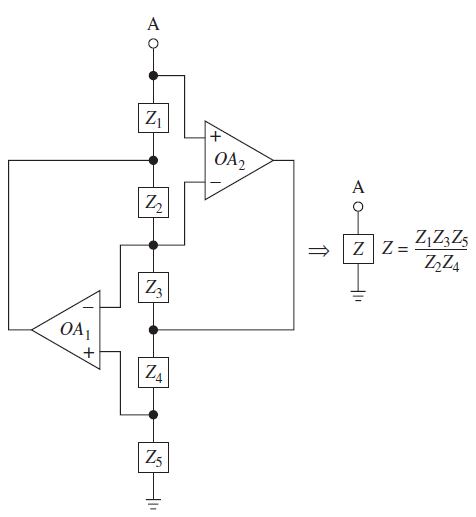
\includegraphics[width=0.6\textwidth]{Imagenes/gic.PNG}
	\caption{Convertidor generalizado de impedancia puesto a tierra[1].}
	\label{fig:gic}
\end{figure}

Estos circuitos están compuestos solamente por resistores, capacitores y amplificadores operacionales, por lo que sobresalen en su uso como emuladores de inductores o capacitores de gran capacidad.

\begin{figure}[H]
	\centering
	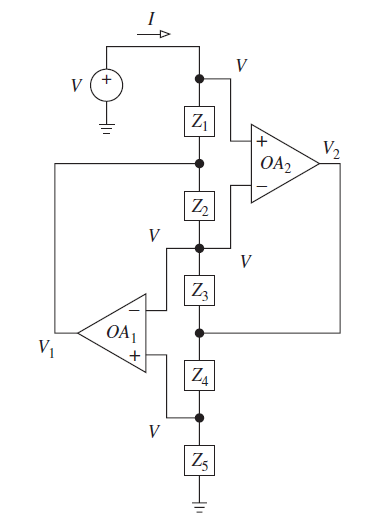
\includegraphics[width=0.5\textwidth]{Imagenes/gic_zin.PNG}
	\caption{Obtención de la impedancia de entrada del convertidor generalizado de impedancia puesto a tierra[2].}
	\label{fig:gic_zin}
\end{figure}

Para obtener la impedancia de entrada del GIC basta solamente calcular la corriente de entrada y utilizar la ley de nodos de Kirchhoff en los nodos de potencial V.

\begin{equation}
\frac{V-V_1}{Z_1}=I
\label{gic_zin_1}
\end{equation}

\begin{equation}
\frac{V_1-V}{Z_2} = \frac{V-V_2}{Z_3}
\label{gic_zin_2}
\end{equation}

\begin{equation}
\frac{V_2-V}{Z_4} = \frac{V}{Z_5}
\label{gic_zin_3}
\end{equation}

Utilizando (\ref{gic_zin_1}), (\ref{gic_zin_2}) y (\ref{gic_zin_3}) se llega finalmente a

\begin{equation}
Z_{in} = \frac{Z_1 Z_3 Z_5}{Z_2 Z_4}
\label{grounded_gic_zin}
\end{equation}

Esto demuestra que un GIC se puede utilizar para emular la impedancia que se desee, eligiendo convenientemente las impedancias $Z_1, \ Z_2, \ Z_3, \ Z_4 \ y \ Z_5$ dentro de las limitaciones que este posee.

\begin{figure}[H]
	\centering
	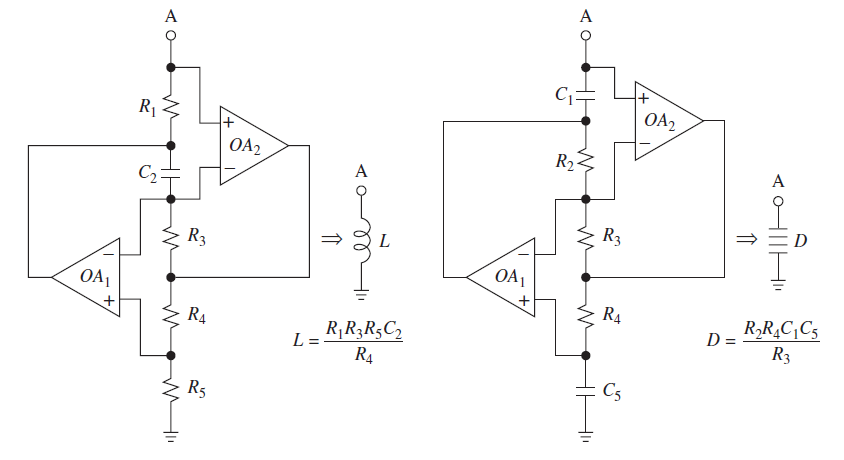
\includegraphics[width=1\textwidth]{Imagenes/gic_ind_fndr.PNG}
	\caption{Utilización de GICs para emular una inductancia a la izquierda y realizar un FNDR o elemento D a la derecha[3].}
	\label{fig:gic_ind_fndr}
\end{figure}

Como se puede observar en la Figura (\ref{fig:gic_ind_fndr}), dos implementaciones muy utilizadas de los GICs puestos a tierra son la de un inductor o un FNDR. Sin embargo, estas implementaciones poseen varias limitaciones a la hora de realizar el diseño de un filtro ya que por la naturaleza interna de los amplificadores operacionales, se debe tener en cuenta que debe haber un camino para la continua que pueda ser utilizada para polarizar correctamente los transistores en el interior de los operacionales. En el siguiente circuito se analizará e implementará un filtro activo con un GIC que no está no puesto a tierra.


\subsection{Análisis del Circuito}

En una primera instancia, se puede observar en la Figura (\ref{fig:circ_redibujado}) como el circuito a analizar consiste de un filtro de primer orden compuesto por un convertidor generalizado de impedancia cuya salida se encuentra realimentada a la entrada. Si bien la elección de las impedancias del GIC sugieren que este se comporta como un inductor y que el filtro será de segundo orden, la realimentación por la resistencia $R_8$ al potencial de entrada exige un análisis detallado de la función transferencia del circuito. Este será el primer paso a tomar en el análisis del filtro.

\subsubsection{Análisis de la Función Transferencia}
\label{sec:fun_trans}
Para realizar el análisis de la función transferencia se consideran los amplificadores operacionales como ideales.

\begin{figure}[H]
\centering
\scalebox{0.5}{
\begin{circuitikz}
\draw

(5, 0) node[label=north:$V_1$](V1){} %Punto inicial, mas o menos centrado horizontalmente
	to[short] ++ (-3,0)
	to[R, l=$R_6$, *-] ++ (0, -2)
	node[ground]{}
	to[open] ++ (0, 2)
	to[short] ++ (-1, 0)
	to[C, l_=$C_6$, *-] ++ (0, -2)
	node[ground]{}
	to[open] ++ (0, 2)
	to[short] ++ (-1, 0)
	node[](R7_right){}
	to[C, l=$C_7$, *-*] ++ (-2, 0)
	node[](R7_left){}
	to[short] ++ (-1,0)
	node[](gic_loop){}
	to[short] ++ (-1,0)
	to[V, l=$V_i$] ++ (0, -2)
	node[ground]{}

(R7_left) to[short] ++ (0, 1)
	to[R, l=$R_7$] ++ (2, 0)
	to[short] (R7_right)	

(V1) to[R, l=$R_1$] ++ (0, -2)
	node[label = east:$V_2$](V2){}
	
(V2) to[C, l=$C_2$] ++ (0, -2)
	node[](V3){}
	to[open] ++ (-0.5, 0.5)
	node[](){$V_3$}
	to[open] ++ (0.5, -0.5)

(V3) to[R, l=$R_3$] ++ (0, -2)
	node[label=west:$V_4$](V4){}
	
(V4) to[R, l=$R_4$] ++ (0, -2)
	node[label=east:$V_5$](V5){}

(V5) to[R, l=$R_8$] ++ (0,-2)
	to[short] ++ (-8, 0)
	to[short, -*] (gic_loop)

(V2) to[open] ++ (3, 0)
	node[op amp, yscale=-1](opamp){}

(opamp.+) to[short] ++ (-0.5, 0)
	to[short] ++ (0, 1.5)
	to[short, -*] (V1)
	
(opamp.-) to[short] ++ (-0.5, 0)
	to[short] ++ (0, -1.5)
	to[short, -*] (V3)

(opamp.out) to[short] ++ (1, 0)
	node[label=east:$V_{out}$](Vout){}
	to[short] ++ (0, -4)
	to[short, -*] (V4)
	
(V4) ++ (-3, 0) node[op amp, xscale=-1](opamp2){}

(opamp2.+) to[short] ++ (0.5, 0)
	to[short] ++ (0, -1.5)
	to[short, -*] (V5)
	
(opamp2.-) to[short] ++ (0.5, 0)
	to[short] ++ (0, 1.5)
	to[short, -*] (V3)
	
(opamp2.out) to[short] ++ (0, 2.5)
	to[short] ++ (2.5, 0)
	to[short] ++ (0, 1.5)
	to[short, -*] (V2)

;
\end{circuitikz}
}
\caption{Circuito a analizar redibujado para facilitar la obtención de la función transferencia.}
\label{fig:circ_redibujado}
\end{figure}

Redibujando adecuadamente el circuito, se puede observar como los operacionales mantienen a sus entradas el mismo potencial. Como paso siguiente, y para utilizar el método de nodos en aquellos que son mantenidos a un mismo potencial, se debe dibujar nuevamente al circuito aplicando el teorema de Thévenin entre los nodos $V_1$ y tierra. Para esto, se desconecta la realimentación por medio de la resistencia $R_8$ teniendo en cuenta los efectos que esta producen sobre el circuito.

\begin{figure}[H]
\centering
\begin{subfigure}[t]{0.49\textwidth}
\centering
\scalebox{0.4}{
\begin{circuitikz}

\draw

(5, 0) node[label=north:$V_1$](V1){} %Punto inicial, mas o menos centrado horizontalmente
	to[short] ++ (-3,0)
	to[R, l=$R_6$, *-] ++ (0, -2)
	node[ground]{}
	to[open] ++ (0, 2)
	to[short] ++ (-1, 0)
	to[C, l_=$C_6$, *-] ++ (0, -2)
	node[ground]{}
	to[open] ++ (0, 2)
	to[short] ++ (-1, 0)
	node[](R7_right){}
	to[C, l=$C_7$, *-*] ++ (-2, 0)
	node[](R7_left){}
	to[short] ++ (-1,0)
	node[](gic_loop){}
	to[short] ++ (-1,0)
	to[V, l=$V_i$] ++ (0, -2)
	node[ground]{}

(R7_left) to[short] ++ (0, 1)
	to[R, l=$R_7$] ++ (2, 0)
	to[short] (R7_right)	

(V1) to[R, l=$R_1$] ++ (0, -2)
	node[label = east:$V_2$](V2){}
	
(V2) to[C, l=$C_2$] ++ (0, -2)
	node[](V3){}
	to[open] ++ (-0.5, 0.5)
	node[](){$V_3$}
	to[open] ++ (0.5, -0.5)

(V3) to[R, l=$R_3$] ++ (0, -2)
	node[label=west:$V_4$](V4){}
	
(V4) to[R, l=$R_4$] ++ (0, -2)
	node[label=east:$V_5$](V5){}

(V5) to[R, l=$R_8$] ++ (0,-2)
	to[short] ++ (-7, 0)
	to[short, -*] ++ (0, 5)
	to[V, l=$V_i$] ++ (-2, 0)
	to[short] ++ (0, -1)
	node[ground](){}

(V2) to[open] ++ (3, 0)
	node[op amp, yscale=-1](opamp){}

(opamp.+) to[short] ++ (-0.5, 0)
	to[short] ++ (0, 1.5)
	to[short, -*] (V1)
	
(opamp.-) to[short] ++ (-0.5, 0)
	to[short] ++ (0, -1.5)
	to[short, -*] (V3)

(opamp.out) to[short] ++ (1, 0)
	node[label=east:$V_{out}$](Vout){}
	to[short] ++ (0, -4)
	to[short, -*] (V4)
	
(V4) ++ (-3, 0) node[op amp, xscale=-1](opamp2){}

(opamp2.+) to[short] ++ (0.5, 0)
	to[short] ++ (0, -1.5)
	to[short, -*] (V5)
	
(opamp2.-) to[short] ++ (0.5, 0)
	to[short] ++ (0, 1.5)
	to[short, -*] (V3)
	
(opamp2.out) to[short] ++ (0, 2.5)
	to[short] ++ (2.5, 0)
	to[short] ++ (0, 1.5)
	to[short, -*] (V2)

;

\end{circuitikz}
}
\caption{Circuito redibujado.}\label{fig:circ_redibujado_2}
\end{subfigure}
\begin{subfigure}[t]{0.49\textwidth}
\centering
\scalebox{0.6}{
\begin{circuitikz}
 
 \draw

(0,0) node[label=north:$V_1$](V1){}
	to[short, *-] ++ (-1, 0)
	to[R, l=$R_6$] ++ (0, -2)
	node[ground](){}
	to[open] ++ (0, 2)
	to[short, *-*] ++ (-1, 0)
	to[C, l_=$C_6$] ++ (0,-2)
	node[ground](){}
	to[open] ++ (0, 2)
	to[short] ++ (-1, 0)
	to[C, l=$C_7$, *-*] ++ (-2, 0)
	to[short] ++ (0, 1)
	to[R, l=$R_7$] ++ (2, 0)
	to[short] ++ (0, -1)
	to[open] ++ (-2, 0)
	to[short] ++ (-1, 0)
	to[V, l=$V_i$] ++ (0, -2)
	node[ground](){}

;
 
\end{circuitikz}
}
\caption{Circuito para el análisis de Thévenin}
\label{fig:circ_thevenin}
\end{subfigure}
\end{figure}

Se puede observar en la Figura (\ref{fig:circ_thevenin}) como la tensión de Thévenin será el divisor resistivo entre las impedancias equivalentes $Z_6$ y $Z_7$, siendo estas el resultado del paralelo entre $R_6$ y $C_6$ y entre $R_7$ y $C_7$ respectivamente, mientras que la impedancia de Thévenin será el paralelo entre ambas impedancias equivalentes. Resulta entonces:

\begin{equation}
V_{Th} = V_i \cdot \frac{\left(R_6 // \frac{1}{SC_6}\right)}{\left(R_6 // \frac{1}{SC_6}\right) + \left(R_7 // \frac{1}{SC_7}\right)}
\end{equation}

\begin{equation}
R_{Th} = \left(R_6 // \frac{1}{SC_6}\right) // \left(R_7 // \frac{1}{SC_7}\right)
\end{equation}

Finalmente, con las ecuaciones obtenidas habiendo aplicado el teorema de Thévenin, se aplica el método de los nodos en aquellos cuyo potencial se mantiene igual por los operacionales, resultando en:

\begin{equation}
V_1=V_3=V_5=V_A
\label{eq:circ_trans1}
\end{equation}

\begin{equation}
\frac{V_{out} - V_A}{R_4} = \frac{V_A-V_i}{R8}
\label{eq:circ_trans2}
\end{equation}

\begin{equation}
\frac{V_2 - V_A}{\frac{1}{SC_2}} = \frac{V_A-V_{out}}{R_3}
\label{eq:circ_trans3}
\end{equation}

\begin{equation}
\frac{V_i \cdot \frac{\left(R_6 // \frac{1}{SC_6}\right)}{\left(R_6 // \frac{1}{SC_6}\right) + \left(R_7 // \frac{1}{SC_7}\right)} - V_A}{\left(R_6 // \frac{1}{SC_6}\right) // \left(R_7 // \frac{1}{SC_7}\right)} = \frac{V_A-V_2}{R_1}
\label{eq:circ_trans4}
\end{equation} \\

A partir de (\ref{eq:circ_trans1}), (\ref{eq:circ_trans2}), (\ref{eq:circ_trans3}) y (\ref{eq:circ_trans4}) se obtiene:

\begin{equation}
\hspace{-0.5cm}
\frac{V_{out}}{V_i} = \frac{S^2 C_2 R_1 R_3 R_6 R_7 (-C_6 R_4 + C_7 R_8) + S C_2 R_1 R_3 (R_6 R_8 - R_4 R_7) + R_4 R_6 R_7}{S^2 C_2 R_1 R_3 R_6 R_7 R_8 (C_6 + C_7)+S C_2 R_1 R_3 R_8 (R_7 + R_6) + R_4 R_6 R_7}
\label{circ_trans}
\end{equation}

\subsubsection{Análisis de los Componentes}
	
A continuación se hace un breve análisis de la elección de los valores de los componentes y de la funcionalidad de algunos de estos.

\subsubsection{Elección de Componentes y Diseño}
\label{sec:eleccion_componentes}

Utilizando las consideraciones de diseño del circuito de low-pass notch:
$$R_1=R_3=R_4=R_8=R \ \ \ ; \ \ \ R_6=R_7=2QR$$
$$C_2=C \ \ \ ; \ \ \ C_6=(1-\frac{1}{k^2})\frac{C}{2}  \ \ \ ; \ \ \ C_7=(1+\frac{1}{k^2})\frac{C}{2}$$
$$k=\left(\frac{\omega_z}{\omega_p} \right) > 1$$

Se logra obtener la siguiente expresión para el circuito:

\begin{equation}
\frac{Vo}{Vi} = \frac{\left(\frac{S}{\frac{k}{C R}}\right)^2 + 1}{\left( \frac{S}{\frac{1}{CR}} \right)^2+\frac{SCR}{Q} + 1}
\label{circ_trans_simple}
\end{equation}

Finalmente utilizando las consideraciones de los valores de los componentes:
\begin{table}[H]
\centering
\begin{tabular}{@{}ccc@{}}
\toprule
$\omega_p$ & Q & $\omega_z$ \\ \midrule
13.000 $\frac{rad}{s}$ & 2 & $\sqrt{2}*\omega_p \frac{rad}{s}$ \\ \bottomrule
\end{tabular}
\end{table}
Se logra obtener el valor de k:

\begin{equation}
k = \sqrt{2}
\end{equation}

Considerando que hay una mayor facilidad de obtener resistencias de distintos valores que capacitores, se logra obtener la relación que vincula el valor de la resistencia R en función de la capacitancia C elegida:

\begin{equation}
R = \frac{\left(\frac{1}{13000}\right) \frac{s}{rad}}{C}
\end{equation}

Como se desean poseer resistencias pequeñas, ya que el ruido es proporcional a estas, se eligió un valor comercial para la capacitancia C de tal manera que la resistencia R sea del orden de los $10k\Omega$.

$$C=15nF \rightarrow R=5128.2\Omega$$

Es así que quedan fijados los valores de todos los componentes del circuito. A continuación se muestra una tabla con los valores que se deben utilizar, los nominales que se utilizaron en la implementación y los reales de dichos componentes.

\begin{table}[H]
\centering
\begin{tabular}{@{}ccccc@{}}
\toprule
Componente & Valor Teórico & Implementación & Valor Final & Error \\ \midrule
$C_2$ & $15nF$ & $15nF$ & $15nF$ & $0\%$ \\
$C_7$ & $11.25nF$ & $10nF//1.2nF$ & $11.2nF$ & $0.40\%$ \\
$C_6$ & $3.75nF$ & $3.3nF//470pF$ & $3.77nF$ & $0,53\%$\\
$R_{1,3,4,8}$ & $5128.2 \Omega$ & $12K\Omega//9K1\Omega$ & $5175.35 \Omega$ & $0,92\%$ \\
$R_{6,7}$ & $20512.82 \Omega$ & $330K\Omega//22K\Omega$ & $20625\Omega$ & $0,55\%$ \\ \bottomrule
\end{tabular}
\caption{Valores comerciales finales utilizados.}
\label{Tab:valores}
\end{table}

Con estos valores se graficó el Bode en amplitud y fase del filtro:

\begin{figure}[H]
	\centering
	\begin{subfigure}[t]{0.49\textwidth}
	\hspace*{-2cm}
	\centering
		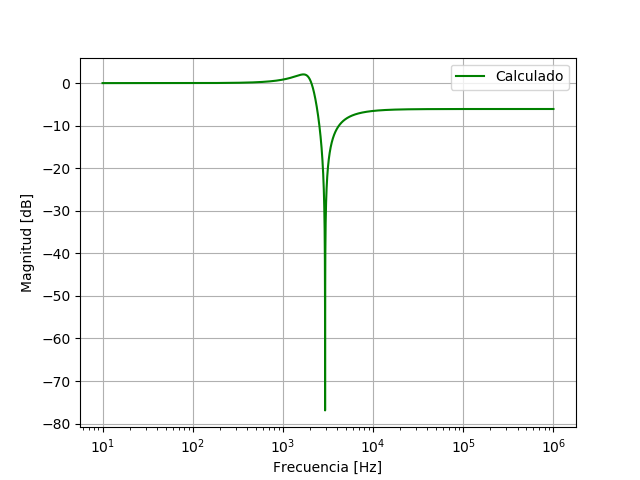
\includegraphics[width=1.3\textwidth]{Imagenes/bodemag_calc.png}
	\end{subfigure}
	\begin{subfigure}[t]{0.49\textwidth}
	\centering
		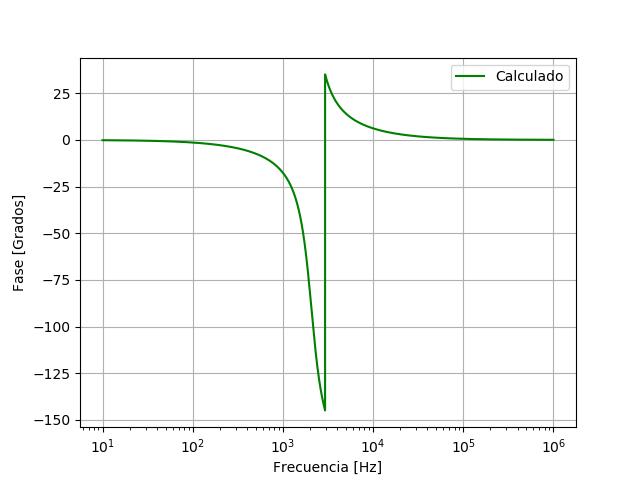
\includegraphics[width=1.3\textwidth]{Imagenes/bodefase_calc.png}
	\end{subfigure}
	\label{fig:bode_calc}
	\caption{Gráficos de Bode para el filtro con los componentes de valor comercial.}
\end{figure}

A continuación se presenta una tabla con los valores significantes de la respuesta en frecuencia.

\begin{table}[H]
\centering
\begin{tabular}{@{}ccccccc@{}}
\toprule
- & $\omega_z$ & $\omega_p$ & Q & $G_{Banda Pasante}$  & $G_{Notch}$ & $G_{Banda Atenuante}$ \\ \midrule
Valor deseado & $2926Hz$ & $2069Hz$ & $2$ & - & - & - \\
Valor calculado & $2930Hz$ & $2066,3Hz$ & $2.01$ & $0$ & $-76.91dB$ & $-6.08dB$ \\ 
Error & $0.135\%$ & $0.131\%$ & $0.546\%$ & - & - & - \\ \bottomrule
\end{tabular}
\caption{Valores significantes teóricos de la respuesta en frecuencia calculada.}
\label{tab:rta_freq_calc}
\end{table}

\subsubsection{Análisis de Ceros y Polos}

Se realizó un análisis de los ceros y polos de la transferencia ideal calculada tanto con los valores usados en la Tabla (\ref{Tab:valores}) como variando las resistencias $R_6$ y $R_8$.
A continuación se muestran los ceros y polos con los valores de la Tabla (\ref{Tab:valores}).

\begin{figure} [H]
	\centering
	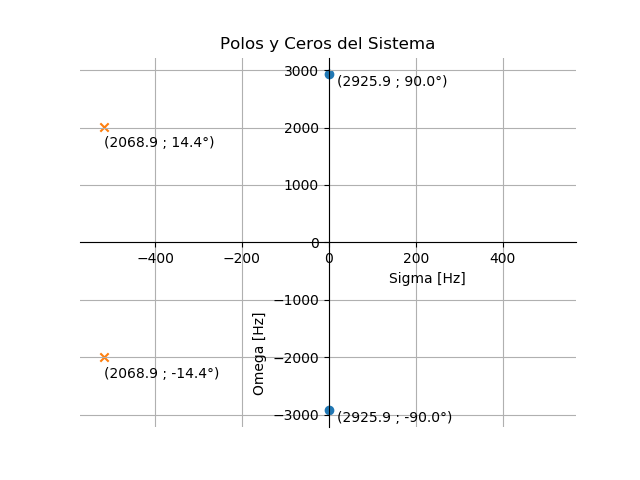
\includegraphics[width=0.8\textwidth]{Imagenes/cerosypolos_calc.PNG}
	\caption{Ceros y polos de la función transferencia ideal del circuito. Módulo y ángulo de cada cero y polo indicado.}
	\label{fig:cerosypolos_calc}
\end{figure}

Se puede observar como los polos y los ceros de la transferencia no se encuentran sobre una circunferencia de mismo radio, sino que los polos tienen una frecuencia de corte menor que la de los ceros. Esto genera que en el diagrama de Bode se encuentre primero el polo y luego el cero, por lo que la curva asintótica permanece por debajo de la línea del cero para las frecuencias mayores a la frecuencia de notch. Se puede contemplar además como los ceros se sitúan sobre el eje imaginario, por lo que el factor de calidad tiende a infinito y genera un gran sobrepico, atenuando casi totalmente las frecuencias cuyo valor sean igual al módulo de los ceros.

Luego, se procede a realizar un análisis del desplazamiento de los polos dadas variaciones en las resistencias $R_6$ y $R_8$. Cabe notar que el color más oscuro corresponde con la posición inicial de los ceros y polos.

\begin{figure}[H]
	\centering
	\begin{subfigure}[t]{0.49\textwidth}
	\hspace*{-2cm}
	\centering
		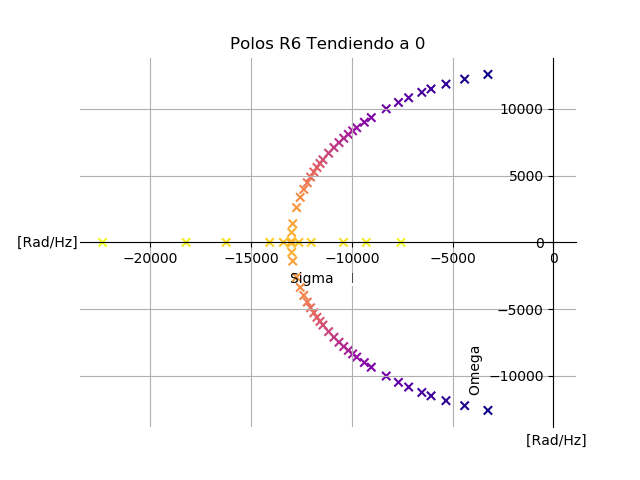
\includegraphics[width=1.2\textwidth]{Imagenes/polosr6a0.png}
	\end{subfigure}
	\begin{subfigure}[t]{0.49\textwidth}
	\centering
		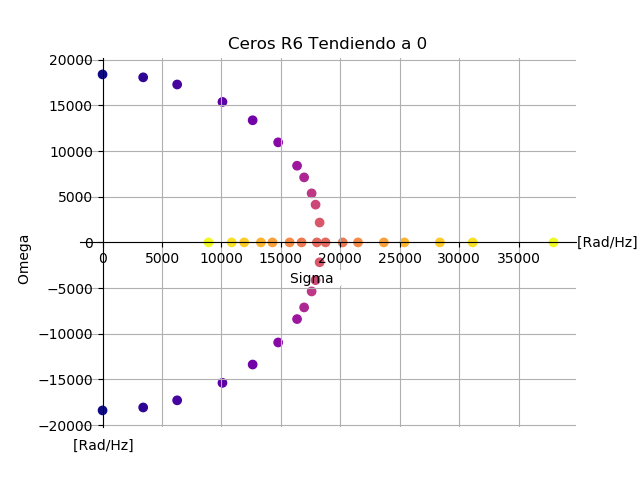
\includegraphics[width=1.2\textwidth]{Imagenes/cerosr6a0.png}
	\end{subfigure}
	\caption{Posición de los ceros y polos de la transferencia cuando $R_6$ parte de su valor original y tiende a cero.}
	\label{fig:r6a0}
\end{figure}

\begin{figure}[H]
	\centering
	\begin{subfigure}[t]{0.49\textwidth}
	\hspace*{-2cm}
	\centering
		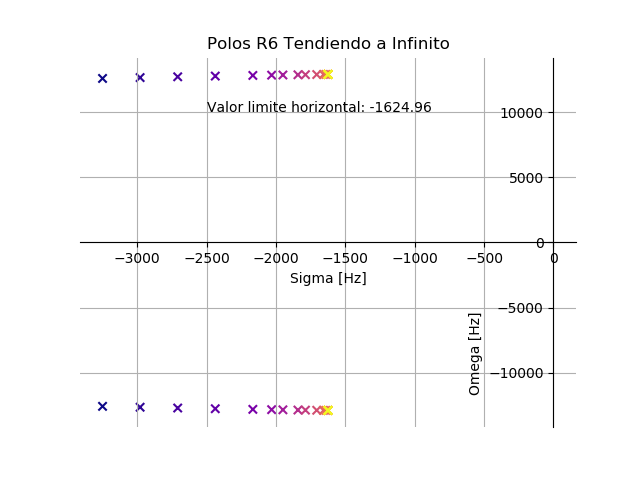
\includegraphics[width=1.2\textwidth]{Imagenes/polosr6ainf.png}
	\end{subfigure}
	\begin{subfigure}[t]{0.49\textwidth}
	\centering
		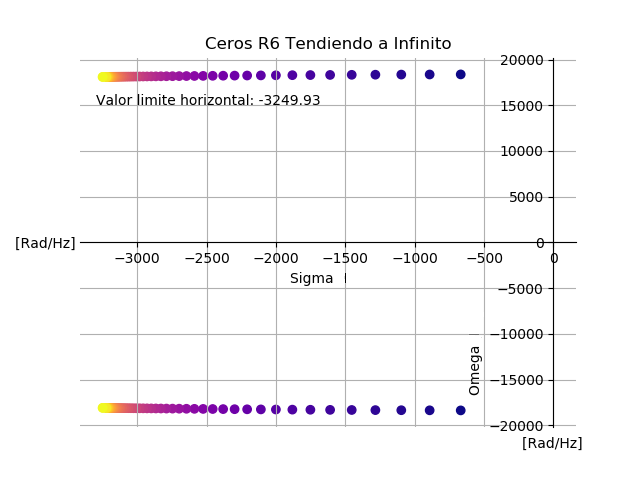
\includegraphics[width=1.2\textwidth]{Imagenes/cerosr6ainf.png}
	\end{subfigure}
	\caption{Posición de los ceros y polos de la transferencia cuando $R_6$ parte de su valor original y tiende a infinito.}
	\label{fig:r6ainf}
\end{figure}

Se puede observar en las Figuras (\ref{fig:r6a0}) y (\ref{fig:r6ainf}) que cambios en la resistencia $R_6$ genera que los ceros y polos no solo se desplacen horizontalmente sino también que estos transicionen de ser complejos conjugados, a estar ubicados en un mismo punto y eventualmente situarse solamente sobre el eje real, apartándose el uno del otro. Además, es observable como si $R_6$ aumenta de su valor original, disminuirá el sobrepico de los ceros y aumentará el sobrepico de los polos. Si $R_6$ tiende a cero, se contempla como baja el factor de calidad de tanto los ceros como los polos, por lo que el filtro pierde su naturaleza de notch y pasa a asemejarse más a la curva asintótica de la transferencia. Con este análisis se puede llegar a la conclusión que la resistencia $R_6$ regula el factor de calidad del circuito.


A continuación se analiza el desplazamiento de los polos variando la resistencia $R_8$. 

\begin{figure}[H]
	\centering
	\begin{subfigure}[t]{0.49\textwidth}
	\hspace*{-2cm}
	\centering
		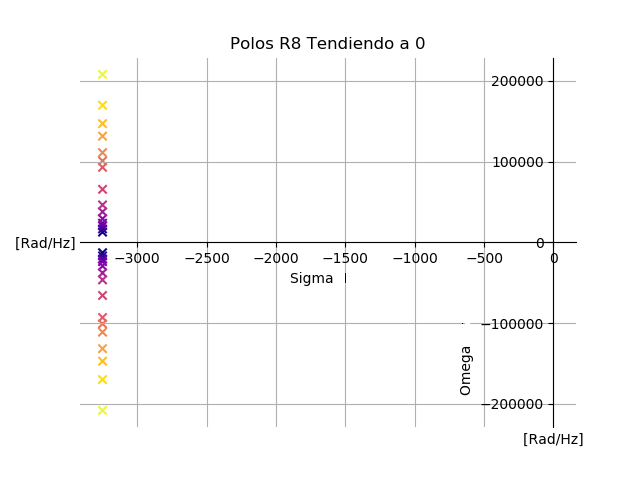
\includegraphics[width=1.2\textwidth]{Imagenes/polosr8a0.png}
	\end{subfigure}
	\begin{subfigure}[t]{0.49\textwidth}
	\centering
		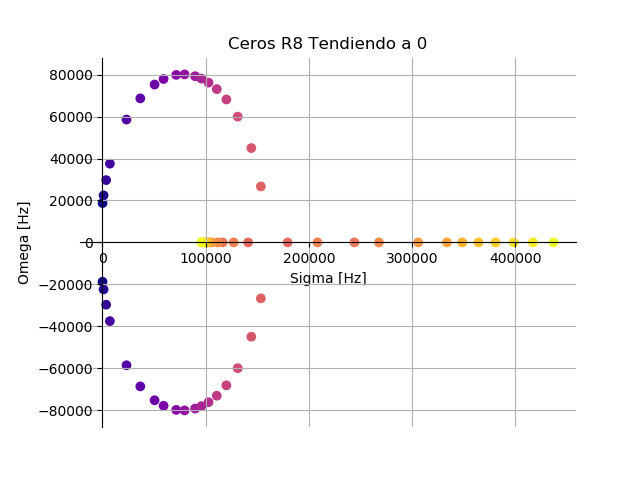
\includegraphics[width=1.2\textwidth]{Imagenes/cerosr8a0.png}
	\end{subfigure}
	\caption{Posición de los ceros y polos de la transferencia cuando $R_8$ parte de su valor original y tiende a cero.}
	\label{fig:r8a0}
\end{figure}

\begin{figure}[H]
	\centering
	\begin{subfigure}[t]{0.49\textwidth}
	\hspace*{-2cm}
	\centering
		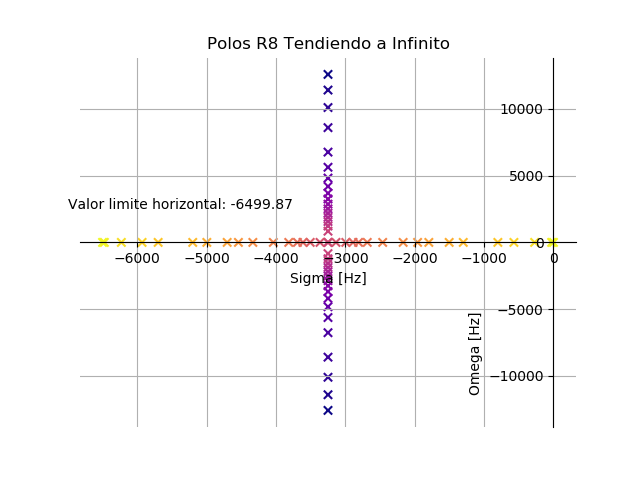
\includegraphics[width=1.2\textwidth]{Imagenes/polosr8ainf.png}
	\end{subfigure}
	\begin{subfigure}[t]{0.49\textwidth}
	\centering
		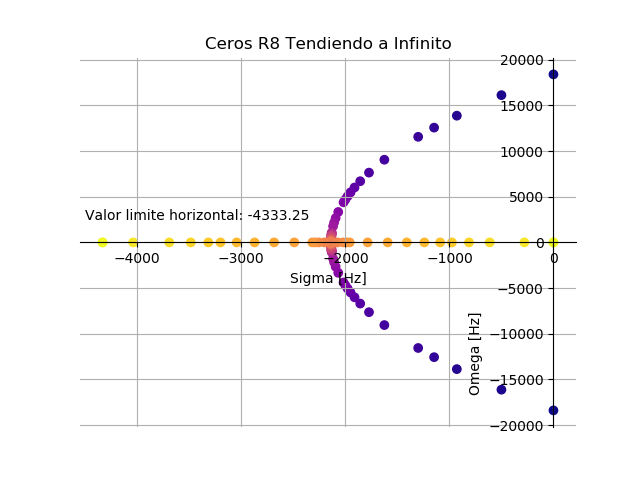
\includegraphics[width=1.2\textwidth]{Imagenes/cerosr8ainf.png}
	\end{subfigure}
	\caption{Posición de los ceros y polos de la transferencia cuando $R_8$ parte de su valor original y tiende a infinito.}
	\label{fig:r8ainf}
\end{figure}

Se contempla en las Figuras (\ref{fig:r8a0}) y (\ref{fig:r8ainf}) como pequeñas variaciones en la resistencia $R_8$ logra generar corrimientos en la frecuencia de notch del circuito, manteniendo aproximadamente su forma. Si las variaciones son muy extremas, se pierde la condición de notch ya que varía el factor de calidad del circuito.

Se puede concluir que la resistencia $R_8$ y sus pares regulan la frecuencia del notch, dentro de ciertos límites en los que la selectividad se conserva aproximadamente.

\subsubsection{Análisis de Sensibilidades}

El análisis de sensibilidades es una herramienta fundamental a la hora de diseñar no solo filtros, sino cualquier circuito electrónico. Este análisis permite conocer cuánto cambia un parámetro fundamental del circuito, como por ejemplo la selectividad, dada una variación en otro de sus parámetros, como por ejemplo una resistencia.

La sensibilidad de un parámetro $y$ respecto a otro parámetro $x$ se calcula como

\begin{equation}
S^y_x = \frac{x}{y} \frac{\partial y}{\partial x}
\end{equation}

Para el análisis de sensibilidades se remite a la función transferencia obtenida en la Sección (\ref{sec:fun_trans}) reescrita a continuación.

\[
\hspace{-0.5cm}
\frac{V_{out}}{V_i} = \frac{S^2 C_2 R_1 R_3 R_6 R_7 (-C_6 R_4 + C_7 R_8) + S C_2 R_1 R_3 (R_6 R_8 - R_4 R_7) + R_4 R_6 R_7}{S^2 C_2 R_1 R_3 R_6 R_7 R_8 (C_6 + C_7)+S C_2 R_1 R_3 R_8 (R_7 + R_6) + R_4 R_6 R_7}
\]

Como primer paso, se realiza un análisis de la sensibilidad de la frecuencia de notch $\omega_z$ en función de los componentes resistivos y capacitivos del circuito.

Considerando que
\begin{equation}
\omega_z = \frac{1}{\sqrt{C_2 R_1 R_3 R_6 R_7 (C_7 R_8 - C_6 R_4)}}
\end{equation}

se halla la derivada parcial de $\omega_z$ respecto de $R_1$ como

\begin{equation}
\frac{\partial \omega_z}{\partial R_1} = -\frac{1}{2} \frac{C_2 R_3 R_6 R_7 (C_7 R_8 - C_6 R_4)}{(C_2 R_1 R_3 R_6 R_7 (C_7 R_8 - C_6 R_4))^{\frac{3}{2}}}
\end{equation}

siendo finalmente la sensibilidad de la frecuencia de notch respecto de la resistencia $R_1$

\begin{equation}
S^{\omega_z}_{R_1} = - \frac{1}{2}  R_1 \sqrt{C_2 R_1 R_3 R_6 R_7 (C_7 R_8 - C_6 R_4)} \frac{C_2 R_3 R_6 R_7 (C_7 R_8 - C_6 R_4)}{(C_2 R_1 R_3 R_6 R_7 (C_7 R_8 - C_6 R_4))^{\frac{3}{2}}} = -\frac{1}{2}
\end{equation}

De forma análoga se calculó el resto de las sensibilidades de la frecuencia de notch respecto a los componentes resistivos y capacitivos presentados a continuación.

\begin{table}[H]
\centering
\begin{tabular}{@{}ccccccccc@{}}
\toprule
$S^{\omega_z}_{R_1}$ & $S^{\omega_z}_{C_2}$ & $S^{\omega_z}_{R_3}$ & $S^{\omega_z}_{R_4}$ & $S^{\omega_z}_{R_8}$ & $S^{\omega_z}_{R_6}$ & $S^{\omega_z}_{C_6}$ & $S^{\omega_z}_{R_7}$ & $S^{\omega_z}_{C_7}$  \\ \midrule
$-\frac{1}{2}$ & $-\frac{1}{2}$ & $-\frac{1}{2}$ & $\frac{1}{2}\frac{R_4 C_6}{C_7 R_8 - C_6 R_4}$ & $-\frac{1}{2}\frac{R_8 C_7}{C_7 R_8 - C_6 R_4}$ & $-\frac{1}{2}$ & $\frac{1}{2}\frac{R_4 C_6}{C_7 R_8 - C_6 R_4}$ & $-\frac{1}{2}$ & $-\frac{1}{2} \frac{R_8 C_7}{C_7 R_8 - C_6 R_4}$ \\ \bottomrule
\end{tabular}
\caption{Sensibilidades de la frecuencia de notch respecto a los componentes resistivos y capacitivos del circuito.}
\label{tab:sens_wz}
\end{table}

Dadas las sensibilidades obtenidas, se puede observar que solamente cuatro de aquellas son distintas de $\pm \frac{1}{2}$. Si no se tuviesen consideraciones para la implementaciones del circuito, se podría minimizar la sensibilidad de la frecuencia de notch respecto a los capacitores, ya que estos son los que tienen una mayor tolerancia. No obstante, utilizando las consideraciones de la implementación del circuito, sucede que las sensibilidades de $R_4$, $R_8$, $C_6$ y $C_7$ son iguales a $\frac{1}{4}(k^2-1)$ por lo que las sensibilidades respecto a estos componentes pueden llegar a tornarse muy alta cuanto más apartados estén los polos de los ceros en módulo. 

A continuación se presentan las sensibilidades de la frecuencia de corte de los polos en función de los componentes resistivos y capacitivos del circuito.

\begin{table}[H]
\centering
\begin{tabular}{@{}ccccccccc@{}}
\toprule
$S^{\omega_p}_{R_1}$ & $S^{\omega_p}_{C_2}$ & $S^{\omega_p}_{R_3}$ & $S^{\omega_p}_{R_4}$ & $S^{\omega_p}_{R_8}$ & $S^{\omega_p}_{R_6}$ & $S^{\omega_p}_{C_6}$ & $S^{\omega_p}_{R_7}$ & $S^{\omega_p}_{C_7}$  \\ \midrule
$-\frac{1}{2}$ & $-\frac{1}{2}$ & $-\frac{1}{2}$ & $0$ & $-\frac{1}{2}$ & $-\frac{1}{2}$ & $-\frac{1}{2}\frac{C_6}{C_6+C_7}$ & $-\frac{1}{2}$ & $-\frac{1}{2} \frac{C_7}{C_7+ C_6}$ \\ \bottomrule
\end{tabular}
\caption{Sensibilidades de la frecuencia de los polos respecto a los componentes resistivos y capacitivos del circuito.}
\label{tab:sens_wp}
\end{table}

Un resultado interesante es que variaciones en la resistencia $R_4$ no generan cambios en el posicionamiento de los polos, pero si generan cambios en el factor de calidad de ambas singularidades.

Otro resultado que destaca el análisis de las sensibilidades, tanto de los ceros como los polos, es como una variación en la resistencia $R_1$ de influye de misma manera en el posicionamiento de los polos y ceros por igual, por lo que se puede utilizar un preset en el lugar de esta resistencia para finamente calibrar la respuesta del circuito si esta se ve levemente corrida, sin perturbar la ganancia para las altas frecuencias.


El cálculo y la presentación de las sensibilidades de las selectividades de ambas singularidades se omitió por ser de carácter engorroso y resultar en la dependencia de muchos de los parámetros del circuito.

\subsubsection{Elección de los Amplificadores Operacionales}

Al momento de elegir el operacional a utilizar, se tuvo un claro objetivo: mantener las especificaciones del filtro fieles a lo calculado en el mayor rango de frecuencias posible. Es por esto que uno de los principales parámetros a estudiar en la selección del opamp fue el ancho de banda. Cuanto mayor sea este, más fidedigna será la transferencia en las altas frecuencias, ya que los polos del dispositivo estarán ubicados en mayores frecuencias cuanto más alto sea el ancho de banda.

Otro parámetro importante fueron aquellos que permiten lograr obtener una señal de salida con una baja distorsión armónica. En otras palabras, se buscó no deformar alinealmente a la señal de entrada introduciendo armónicos en esta. Para ello, se consideró la utilización de un amplificador operacional con un alto slew rate.

Finalmente se optó por utilizar el integrado TL-082 el cual posee dos amplificadores operacionales dentro. Se decidieron utilizar estos operacionales ya que poseen un slew rate alto ($13\frac{V}{\mu s}$ valor típico) en comparación a otros operacionales, un ancho de banda grande ($3MHz$ valor típico para ganancia unitaria) y además posee transistores de tecnología J-FET a la entrada del dispositivo, por lo que tanto la corriente de bias como la tensión de offset son más bajos que otro operacional con tecnología BJT a la entrada.

\subsection{Simulación del Circuito}
\label{sec:simulacion}

Se realizó la simulación del circuito utilizando el software \textit{LTSpiceXVII}.

\subsubsection{Simulación de la Transferencia}

Se procedió a realizar la simulación del circuito con los valores obtenidos mediante los paralelos en la Tabla (\ref{Tab:valores}). La primera simulación que se observó fue la respuesta en frecuencia.

\begin{figure}[H]
	\centering
	\begin{subfigure}[t]{0.49\textwidth}
	\hspace*{-2cm}
	\centering
		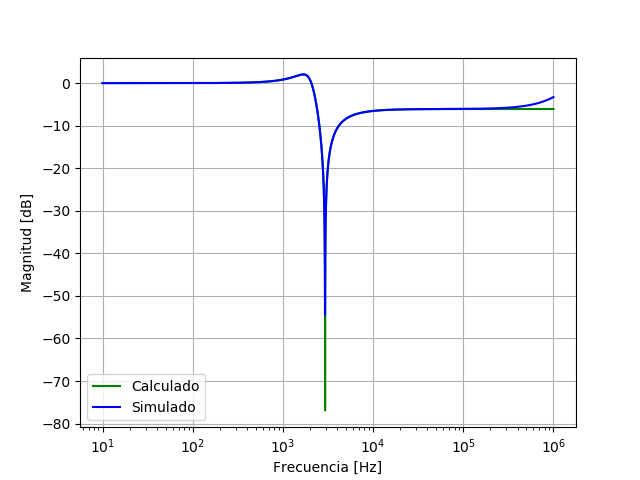
\includegraphics[width=1.3\textwidth]{Imagenes/bodemag_calc_sim.png}
	\end{subfigure}
	\begin{subfigure}[t]{0.49\textwidth}
	\centering
		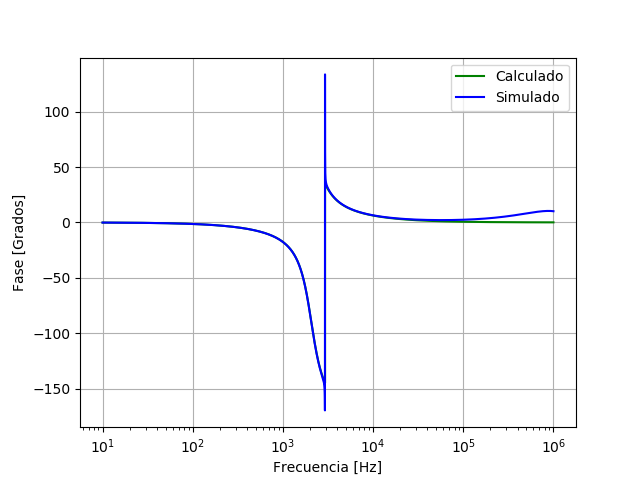
\includegraphics[width=1.3\textwidth]{Imagenes/bodefase_calc_sim.png}
	\end{subfigure}
	\caption{Comparación entre los gráficos de bode simulados y calculados teóricamente.}
	\label{fig:bode_calc_sim}
\end{figure}

Utilizando el operacional elegido en la sección \ref{sec:eleccion_componentes}, se observa una respuesta en frecuencia muy similar a la calculada anteriormente, exceptuando dos puntos de interes.

La ganancia en la frecuencia de notch es mucho menor a la calculada. Esto es algo esperado, ya que muchas cosas que no se tienen en consideración en los cálculos logran llegar a un resultado mucho más ideal que el real.

Respecto a las altas frecuencias, se puede observar una discrepancia entre lo calculado y lo teórico. Esta diferencia es mucho más grande tendiendo a las frecuencias cercanas a los $10MHz$. A continuación se grafica el Bode en fase y magnitud entre las frecuencias de los $100KHz$ y los $100MHz$.

\begin{figure}[H]
	\centering
	\begin{subfigure}[t]{0.49\textwidth}
	\hspace*{-2cm}
	\centering
		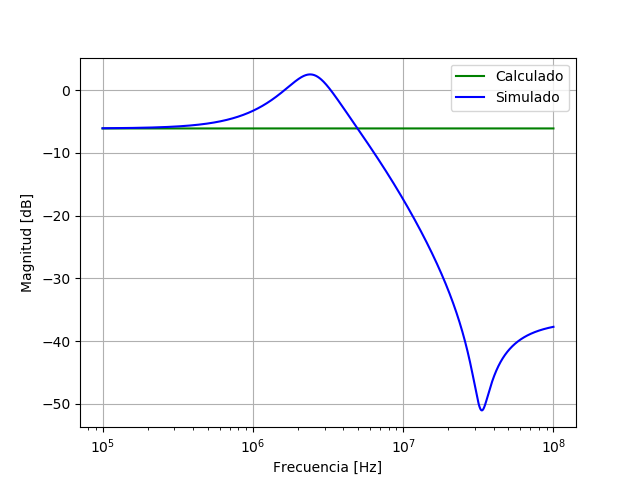
\includegraphics[width=1.3\textwidth]{Imagenes/bodemag_calc_sim_highf.png}
	\end{subfigure}
	\begin{subfigure}[t]{0.49\textwidth}
	\centering
		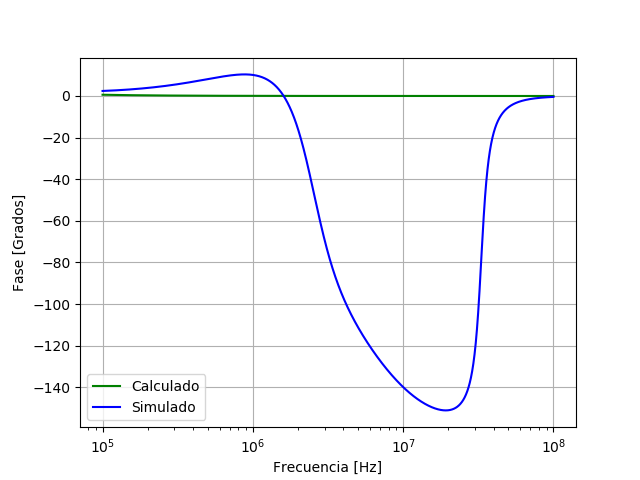
\includegraphics[width=1.3\textwidth]{Imagenes/bodefase_calc_sim_highf.png}
	\end{subfigure}
	\label{fig:bode_calc_sim_highf}
	\caption{Comparación entre los gráficos de bode simulados y calculados teóricamente para las frecuencias mayores a $100KHz$.}
\end{figure}

Si bien el operacional elegido posee un gran ancho de banda para mitigar lo más posible estos problemas a las altas frecuencias, como justificado en la Sección (\ref{sec:eleccion_componentes}), se puede observar que los cálculos realizados con el modelo ideal del operacional poseen una gran diferencia respecto a la simulación, la cual tiene en cuenta los varios polos que posee este dispositivo. Debido a esto, se tendrá en cuenta en la Sección (\ref{sec:limitaciones}) las limitaciones del filtro.

\subsubsection{Simulación de la Impedancia de Entrada y Salida}

Se observó luego la impedancia de entrada y salida del circuito.

\begin{figure}[H]
	\centering
	\begin{subfigure}[t]{0.49\textwidth}
	\hspace*{-2cm}
	\centering
		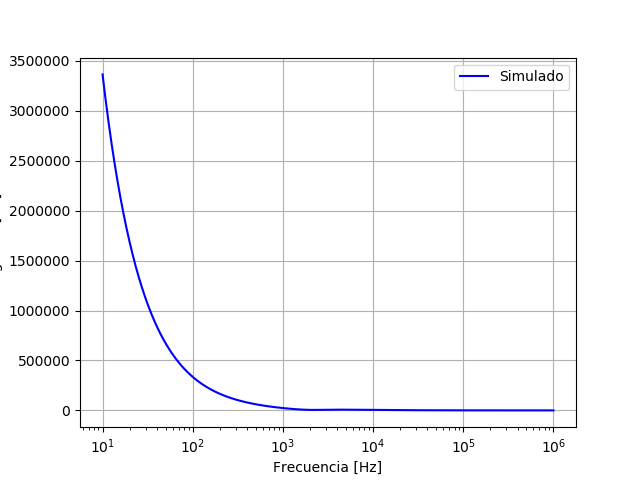
\includegraphics[width=1.3\textwidth]{Imagenes/sim_zin.png}
		\caption{Módulo de la impedancia de entrada.}
	\end{subfigure}
	\begin{subfigure}[t]{0.49\textwidth}
	\centering
		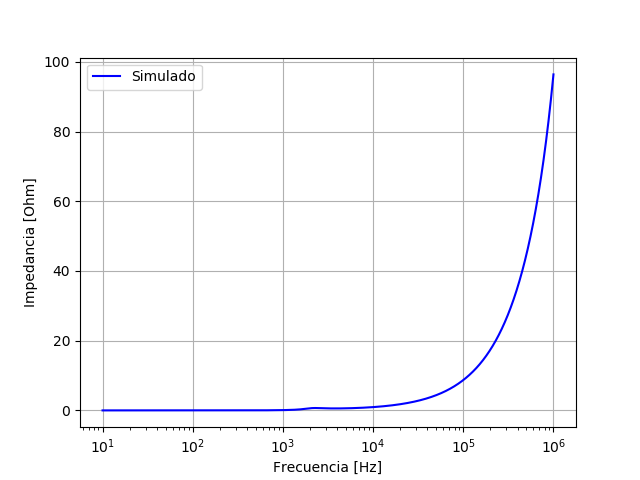
\includegraphics[width=1.3\textwidth]{Imagenes/sim_zout.png}
		\caption{Módulo de la impedancia de salida.}
	\end{subfigure}
	\label{fig:zin_zout}
	\caption{Simulación de la impedancia de entrada y salida del circuito.}
\end{figure}

Se puede ver como tanto la impedancia de entrada como de salida tienden a un valor nulo cuanto más alta la frecuencia. Esto era esperable ya que tanto a la entrada se encuentran dos capacitores cuyo camino a través de ellos lleva a tierra como a la salida se encuentra la impedancia de salida del operacional la cual es muy chica. Esto puede llegar a traer varios problemas a la hora de realizar las mediciones del filtro una vez implementado, por lo que se debe tomar un especial cuidado en esta etapa del análisis. 

\subsubsection{Simulación Montecarlo}
Se utilizó la simulación Montecarlo para observar la dispersión de la respuesta en frecuencia causada por las tolerancias de los componentes. Se utilizó una tolerancia del 5\% para todos los resistores excepto 1\% para las resistencias de 9k1. Para los capacitores se utilizó una tolerancia del 10\%.

\begin{figure}[H]
	\centering
	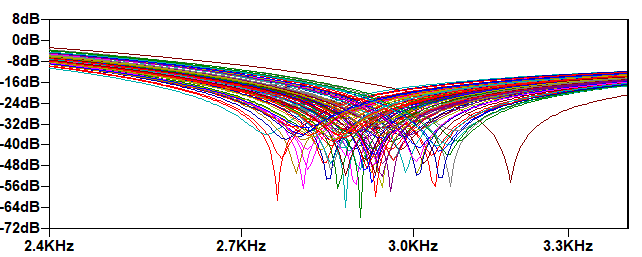
\includegraphics[width=\textwidth]{Imagenes/Montecarlo1.PNG}
	\caption{Simulación de Montecarlo.}
	\label{fig:montecarlo}
\end{figure}

Se puede observar una gran dispersión en la frecuencia de notch de aproximadamente $300Hz$ sin tomar en cuenta el caso de más a la derecha.

\subsection{Implementación del Circuito}
Se implementó el circuito siguiendo las consideraciones y el análisis realizado en la Sección (\ref{sec:eleccion_componentes}). Se decidió utilizar una placa 5x5, resistores al 1\% y 5\% y capacitores de film al 10\%. También se optó por utilizar dos capacitores de desacople de tecnología SMD con un valor de $100nF$ colocados lo más próximo al operacional como posible. 
\subsubsection{Mediciones del Circuito y Análisis de Error}
\subsubsection{Limitaciones del Circuito}
\label{sec:limitaciones}


Se ha recopilado, de la hoja de datos del \href{http://www.ti.com/lit/ds/symlink/tl082.pdf}{TL-082}, los parámetros utilizados en el análisis de las limitacionnes del circuito.

\begin{table}[H]
\centering
\begin{tabular}{@{}ccccc@{}}
\toprule
$V_{CC_{max}}$ & $V_{in_{max}}$ & $BW_{unitgain}$ & $V_{in_{max}}$ dada $V_{CC}$ & Slew Rate (SR)\\ \midrule
$\pm 18V$ & $\pm 15V$ & $3MHz$ & $\approx V_{CC}-1.5V$ & $13\frac{V}{\mu s}$\\ \bottomrule
\end{tabular}
\caption{Datos recopilados de la hoja de datos del TL-082.}
\label{tab:datos_tl082}
\end{table}

Observando la tabla se puede corroborar que la tensión de alimentación no debe sobrepasar los $18V$, mientras que la de entrada no debe sobrepasar los $15V$. Para el análisis de las limitaciones del circuito, sin embargo, se utilizarán $\pm 15V$ de alimentación, valor recomendado por el fabricante.
Luego, teniendo en cuenta que la ganancia máxima del circuito es de $\approx 2dB$, se tiene que

\begin{equation}
	V_{in_{max}} = \frac{V_{CC} - 1.5V}{G_{max}} = \frac{13.5V}{1.26} = 10.72V
\end{equation}

Sin embargo, también se debe de tener en cuenta el slew rate en el análisis de la tensión de entrada máxima.

\begin{equation}
	SR= Max\left( \frac{\partial (G\cdot A\cdot \sin (\omega t))}{\partial t}\right) = V_{in} \cdot \omega \cdot G  
\end{equation}

Primero se analiza la tensión máxima de entrada en la frecuencia de sobrepico ya que esta posee la ganancia más alta.

\begin{equation}
	V_{in_{max}} = \frac{SR}{G_{max}\cdot \omega} = \frac{1.64\cdot 10^6\frac{V}{s}}{1686Hz} = 972.71
\end{equation}

Luego se analiza la tensión máxima de entrada para las frecuencias altas.

\begin{equation}
	V_{in_{max}} = \frac{SR}{G_{Banda Atenuante}\cdot \omega} = \frac{2.01\cdot 10^6\frac{V}{s}}{f}
\end{equation}

Por lo que se graficó la tensión máxima de entrada final en función de la frecuencia tomando en consideración los cálculos previos.

\begin{figure} [H]
	\centering
	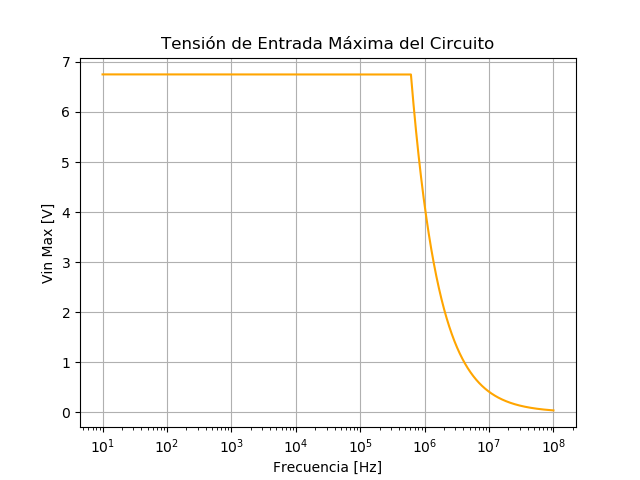
\includegraphics[width=0.7\textwidth]{Imagenes/vin_max.PNG}
	\caption{Tensión de entrada máxima del circuito en función de la frecuencia teniendo en cuenta distorsiones alineales causadas por el operacional.}
	\label{fig:vin_max}
\end{figure}

Luego, el rango de frecuencias en que el circuito opera correctamente, dato conseguido empíricamente, es hasta 1Mhz.


\subsection{Conclusiones}

\subsection{Bibliografía Utilizada}
[1]F. Sergio, Design with operational amplifiers and analog integrated circuits, 4th ed. New York [etc.]: McGraw-Hill, 1988, p. 185.

[2]F. Sergio, Design with operational amplifiers and analog integrated circuits, 4th ed. New York [etc.]: McGraw-Hill, 1988, p. 186.

[3]F. Sergio, Design with operational amplifiers and analog integrated circuits, 4th ed. New York [etc.]: McGraw-Hill, 1988, p. 187.


\end{document}
	\newpage

\section{Introducción a diseño de filtros.}
	\documentclass[a4paper]{article}
\usepackage[utf8]{inputenc}
\usepackage[spanish, es-tabla, es-noshorthands]{babel}
\usepackage[table,xcdraw]{xcolor}
\usepackage[a4paper, footnotesep = 1cm, width=20cm, top=2.5cm, height=25cm, textwidth=18cm, textheight=25cm]{geometry}
%\geometry{showframe}

\usepackage{tikz}
\usepackage{amsmath}
\usepackage{amsfonts}
\usepackage{amssymb}
\usepackage{float}
\usepackage{graphicx}
\usepackage{caption}
\usepackage{subcaption}
\usepackage{multicol}
\usepackage{multirow}
\setlength{\doublerulesep}{\arrayrulewidth}
\usepackage{booktabs}

\usepackage{hyperref}
\hypersetup{
    colorlinks=true,
    linkcolor=blue,
    filecolor=magenta,      
    urlcolor=blue,
    citecolor=blue,    
}

\newcommand{\quotes}[1]{``#1''}
\usepackage{array}
\newcolumntype{C}[1]{>{\centering\let\newline\\\arraybackslash\hspace{0pt}}m{#1}}
\usepackage[american]{circuitikz}
\usetikzlibrary{calc}
\usepackage{fancyhdr}
\usepackage{units} 

\graphicspath{{../Ejercicio-1/}{../Ejercicio-2/}{../Ejercicio-3/}{../Ejercicio-4/}}

\pagestyle{fancy}
\fancyhf{}
\lhead{22.01 Teoría de Circuitos}
\rhead{Mechoulam, Lambertucci, Rodriguez Turco, Londero, Galdeman}
\rfoot{\centering \thepage}
\begin{document}

\subsection{Introducción}

En esta sección se implementó un filtro Band-Pass utilizando una aproximación \textbf{Chebycheff} e implementandola con celdas \textbf{Rauch}, el filtro a diseñar deberá cumplir con la siguiente plantilla.
\begin{table}[H]
\centering
\begin{tabular}{|c|c|}
\hline
$Pendiente$      & -40$\frac{dB}{dec}$           \\ \hline
$f_p$      & 28kHz          \\ \hline
$B$      & $\frac{1}{10}$           \\ \hline
$A_p$      & 3dB               \\ \hline
$Filtro$      & BP              \\ \hline
$|Z_{in}|$ & $\geq 50k \Omega$ \\ \hline
\end{tabular}
\end{table}
\subsection{Aproximación de Chebycheff.}
Para esta sección se utlizó la aproximación de \textbf{Chebyfeff}, además se propuso una plantilla mas restrictiva, con el fin de asegurar el cumplimiento de la original. 

Se despejó el valor de $f_p^+$ y $f_p^-$ 
\begin{align}
f_0^2 = f_p^+ \cdot f_p^- \\
B = \frac{\Delta f_p}{f_0}\\
f_p^+ =29.435 kHz  \ \ \ f_p^- = 26.635 kHz
\end{align}
Luego teniendo en cuenta que la pendiente originalmente es de 40dB por decada se tomo la frecuencia de atenuación acorde  talque mantenga las condiciones de simetría, siendo estas: $f_a^+= 294.35kHz y f_a^- = 2.635kHz$.


Siendo esta la plantilla final.
\begin{table}[H]
\centering
\begin{tabular}{|c|c|}
\hline
$f_s^-$      & 2.6635 kHz          \\ \hline
$f_p^-$      & 26.635 kHz         \\ \hline
$f_p^+$      & 29.435 kHz           \\ \hline
$f_s^+$      & 294.35 kHz          \\ \hline
$A_s$      & 40dB           \\ \hline
$A_p$      & 1dB               \\ \hline
\end{tabular}
\end{table}
Obteniendo la siguiente función transferencia:
\begin{align}
	H(s)=\frac{s}{\left( \frac{s}{23728.54}\right) ^2+s\cdot \frac{23728.54}{3.23}+1}\cdot \frac{s}{\left( \frac{s}{33052.25} \right)^2+s\cdot \frac{33052.25}{3.23}+1}
\end{align}
al cual le corresponde la siguiente respues en frecuencia:

Y el siguiente diagrama de polos y ceros:
\begin{figure}[H]
	\centering
	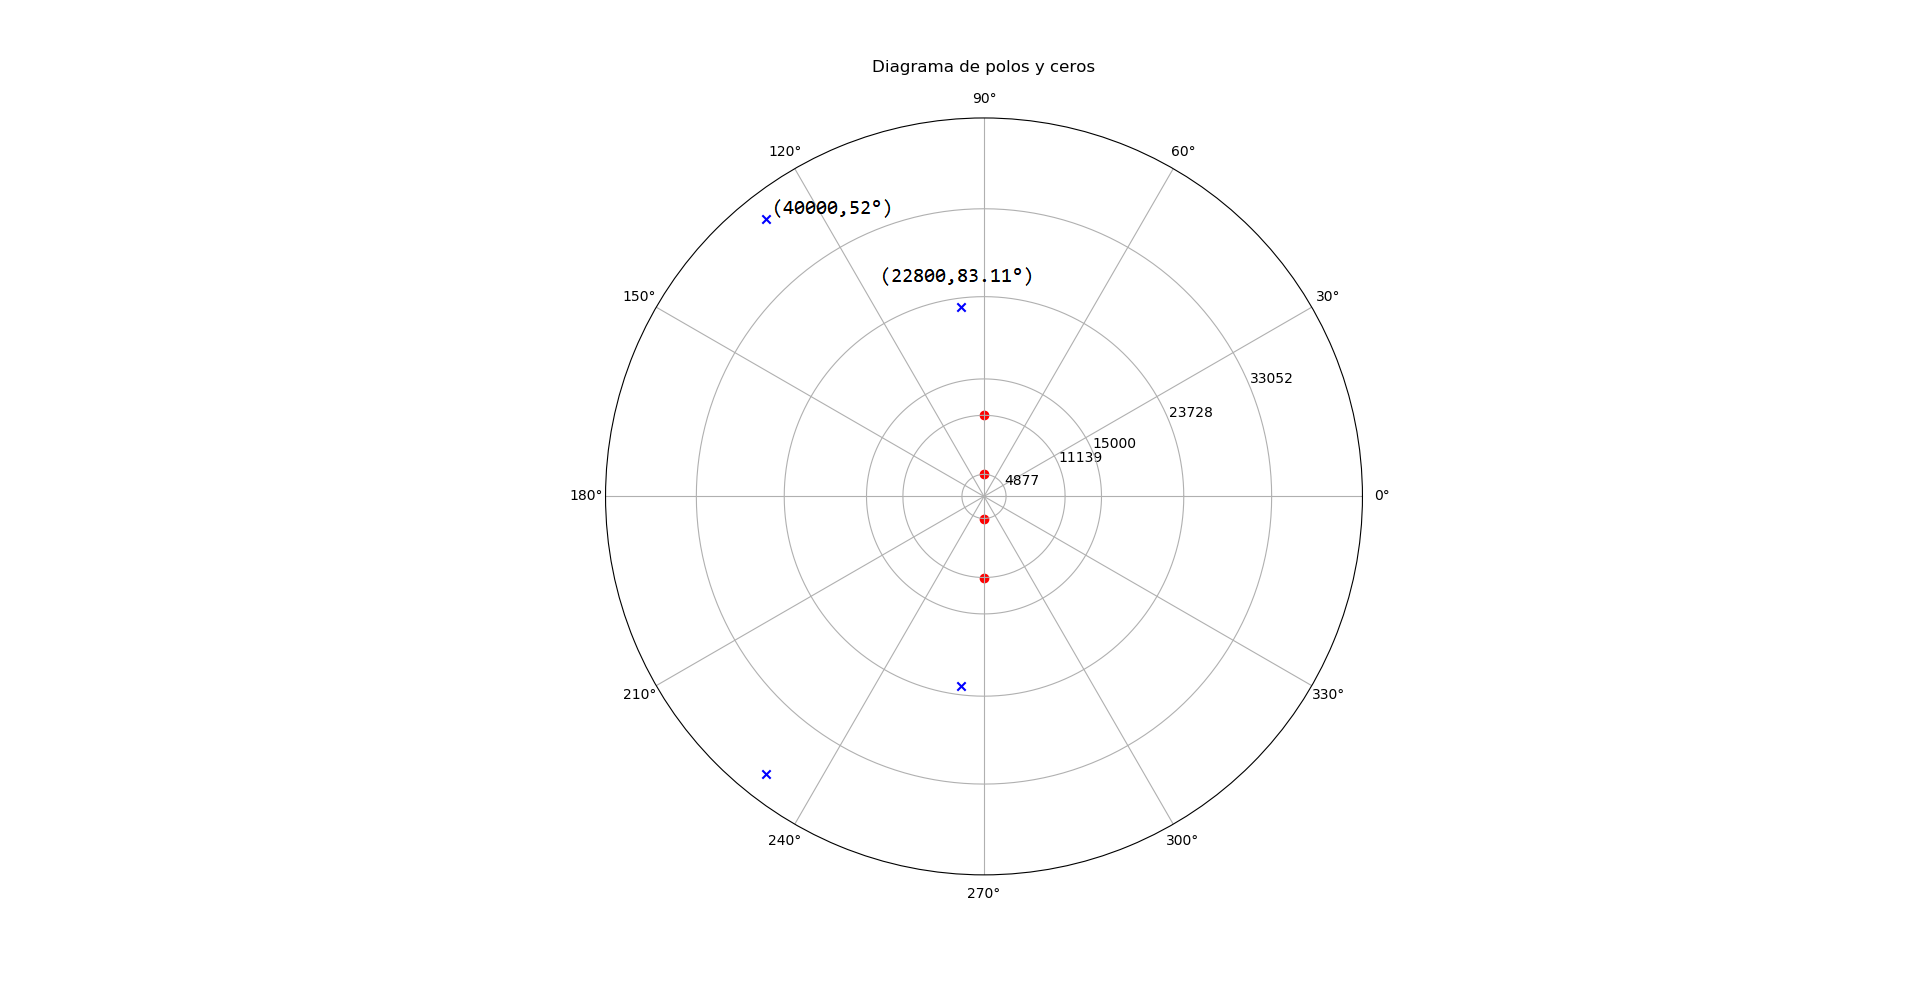
\includegraphics[width=0.5\textwidth]{Imagenes-Ej2/DiagramaPolosYCeros.png}
	\label{fig:stepresponse}
	\caption{Diagrama Polos y Ceros}
\end{figure}

Teniendo los pares de polos conjugados un Q de 3.23	


\subsubsection{Elecciones de diseño}
Se decidió armar etapas con celdas segundo orden en cascada dado a que el orden es 4.
Para la asociación de polos se tomo criterio agrupar cada par de polos con 1 cero , agrupandolos de las siguiente forma.
\begin{figure}[H]
	\centering
	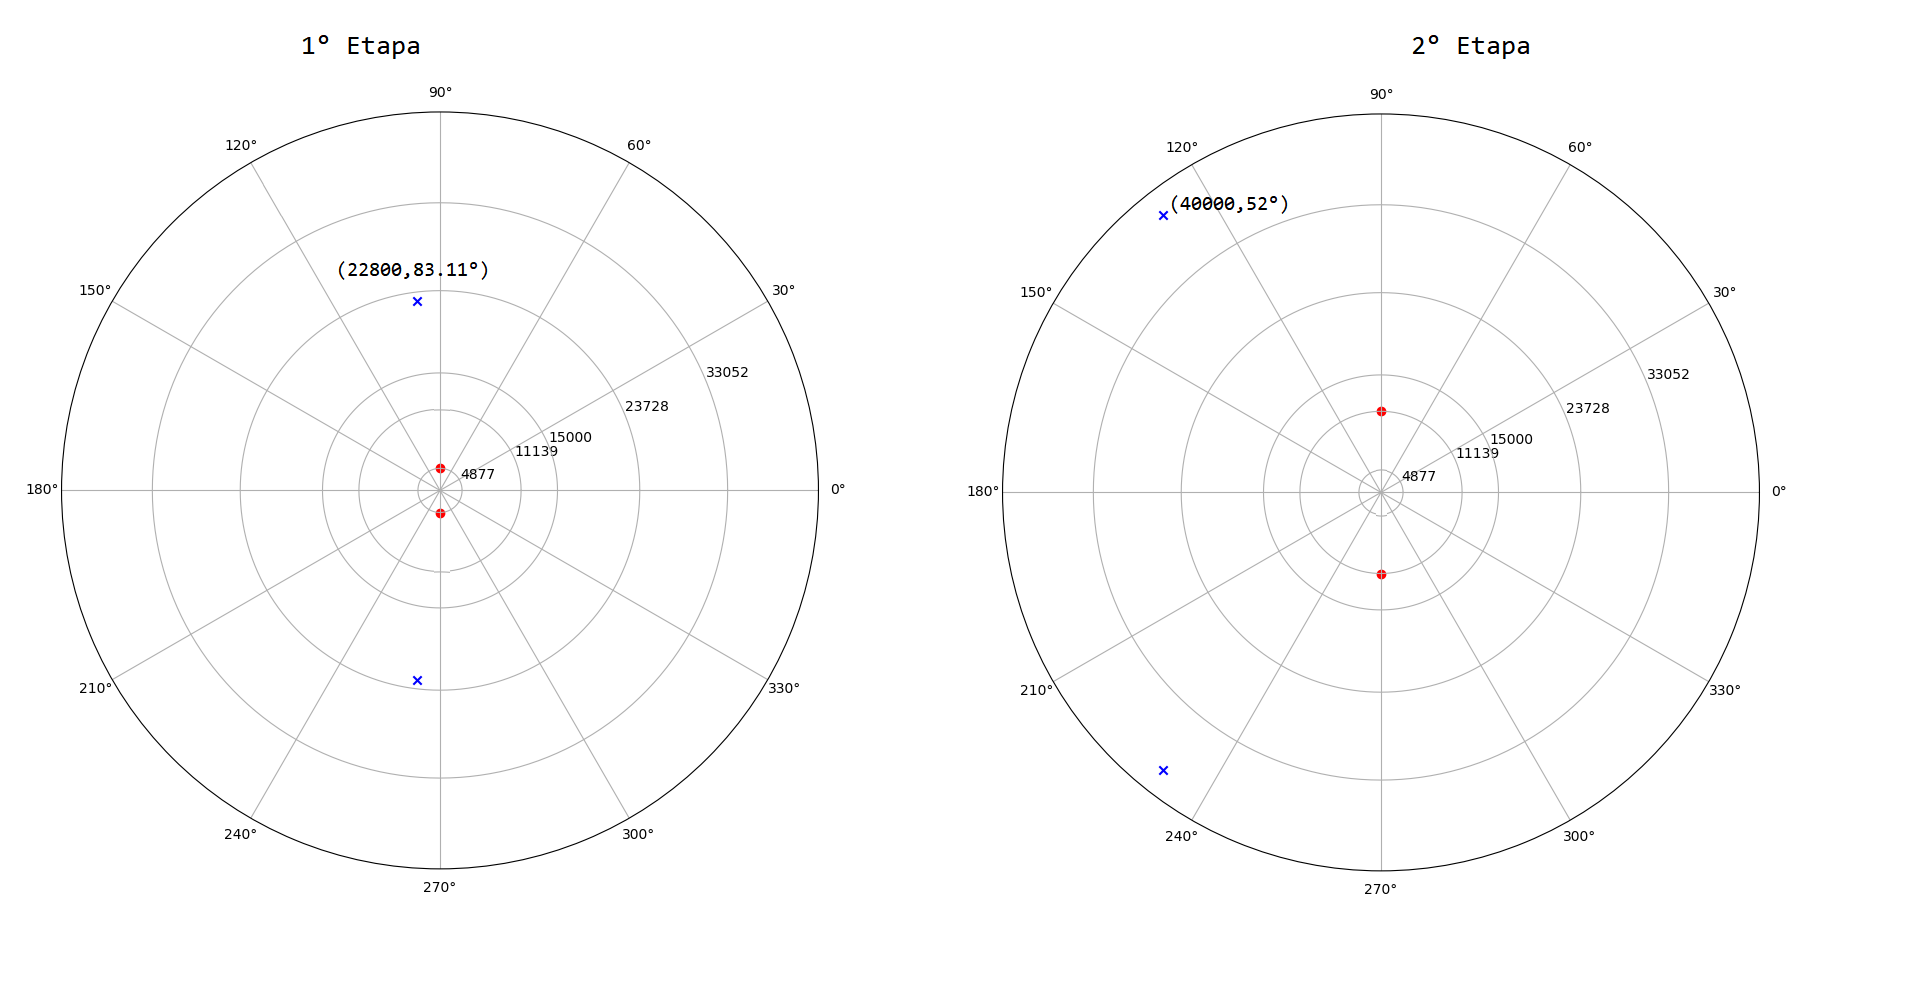
\includegraphics[width=\textwidth]{Imagenes-Ej2/UnionCeros.png}
	\label{fig:CeroPoleUnion}
	\caption{Diagrama Polos y Ceros para cada etapa}
\end{figure}

\subsection{Celda Rauch.}
La celda Rauch es una modificación de la celda Deliyannis-Friend incluyendo uan realimentación positiva.
\begin{figure}[H]
	\centering
	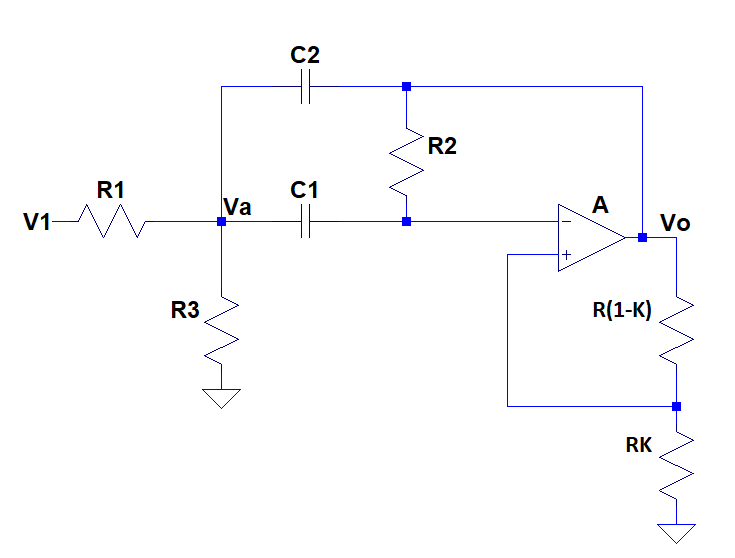
\includegraphics[width=0.5\textwidth]{Imagenes-Ej2/Circuit.PNG}
	\label{fig:graph}
	\caption{Circuito celda Rauch Band-Pass.}
\end{figure}
\subsubsection{Cálculo Analítico}
---
\subsubsection{Elecciones de diseño}

\begin{center}
	\huge{\textcolor{red}{\textbf{Tabla sensibilidades}}}
\end{center}
En base a esta tabla se tomo especial cuidado en la elección de componentes y en el matcheo de impedancias.

Los componentes utilizados fueron los siguientes:
\begin{table}[H]
\centering
\begin{tabular}{lllll}
\multicolumn{1}{c}{Componente} & \multicolumn{1}{c}{1er Etapa} & \multicolumn{1}{c}{Composición} & 2da Etapa      & Composición           \\ \hline
$R_1$                          & $7.3 k\Omega$                 & $10k // 27k  \Omega$            & $5.24 k\Omega$ & $5.6k // 82k  \Omega$ \\
$R_2$                          & $5.56 k\Omega$                & $5.6k // 680k  \Omega$          & $3.99 k\Omega$ & $82 + 3.9k  \Omega$   \\
$R_3$                          & $1.43 k\Omega$                & $1.5 k // 33k  \Omega$          & $1.03k\Omega$  & $27 + 1k  \Omega$     \\
$R_4$                          & $3.49 k\Omega$                & $3.9k // 33k  \Omega$           & $3.49 k\Omega$ & $3.9k // 33k  \Omega$ \\
$R_5$                          & $1 k\Omega$                   & $1 k  \Omega$                   & $1 k\Omega$    & $1 k\Omega$           \\
$C_1$                          & 2.2 nF                        & 2.2 nF                          & 2.2 nF         & 2.2 nF                \\
$C_2$                          & 2.2 nF                        & 2.2 nF                          & 2.2 nF         & 2.2 nF               
\end{tabular}
\end{table}

Se calculó el error porcentual asociado a la aproximación de la resistencias viendose en la siguiente tabla.
\begin{table}[H]
\centering
\begin{tabular}{lll}
\multicolumn{1}{c}{Error Porcentual} & \multicolumn{1}{c}{1er Etapa} & \multicolumn{1}{c}{2da Etapa} \\ \hline
$R_1$                                & 0.1 $\%$                      & $0.038  \%$                   \\
$R_2$                                & 0.1 $\%$                      & 0.2 $\%$                      \\
$R_3$                                & 0.4 $\%$                      & 0.1 $\%$                      \\
$R_4$                                & 0.1 $\%$                      & 0.1 $\%$                      \\
$R_5$                                & $\approx 0 \%$                & $\approx 0 \%$                \\
$C_1$                                & $\approx 0 \%$                & $\approx 0 \%$                \\
$C_1$                                & $\approx 0 \%$                & $\approx 0 \%$               
\end{tabular}
\end{table}

Cabe destacar que todas las imepdancias que fueron colocadas en el circuito fueron elegidas entre varias de su mismo tipo, con la finalidad de poner impedancias que sean realmente de los valores deseados.

\subsubsection{Acoplamiento de Impedancias.}

Para que ambas etapas no se carguen entre si la impedancia de entrada de la segunda etapa debe ser mucho mayor a la de salida de la primera, para lo siguiente se obtuvieron las impedancias de entrada de ambas celdas, incluyendo la de salida de la primera.
\begin{figure}[H]
	\centering
	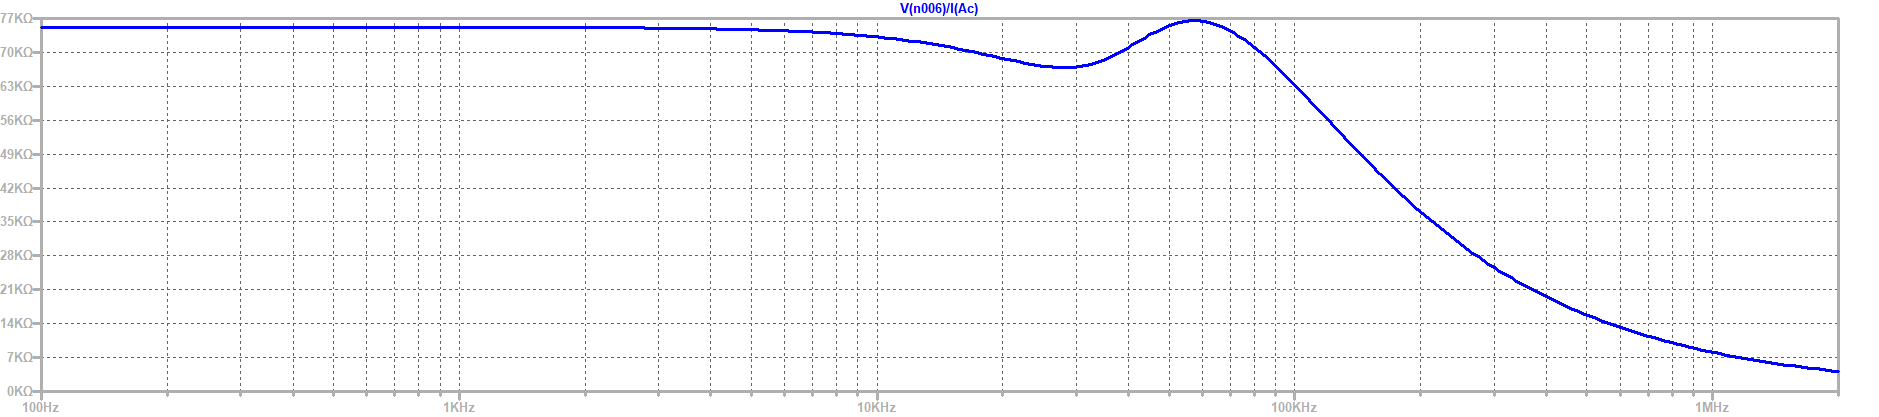
\includegraphics[width=\textwidth]{Imagenes-Ej2/ZinE1.png}
	\label{fig:graph}
	\caption{Impedancia de entrada 1er etapa.}
\end{figure}

\begin{figure}[H]
	\centering
	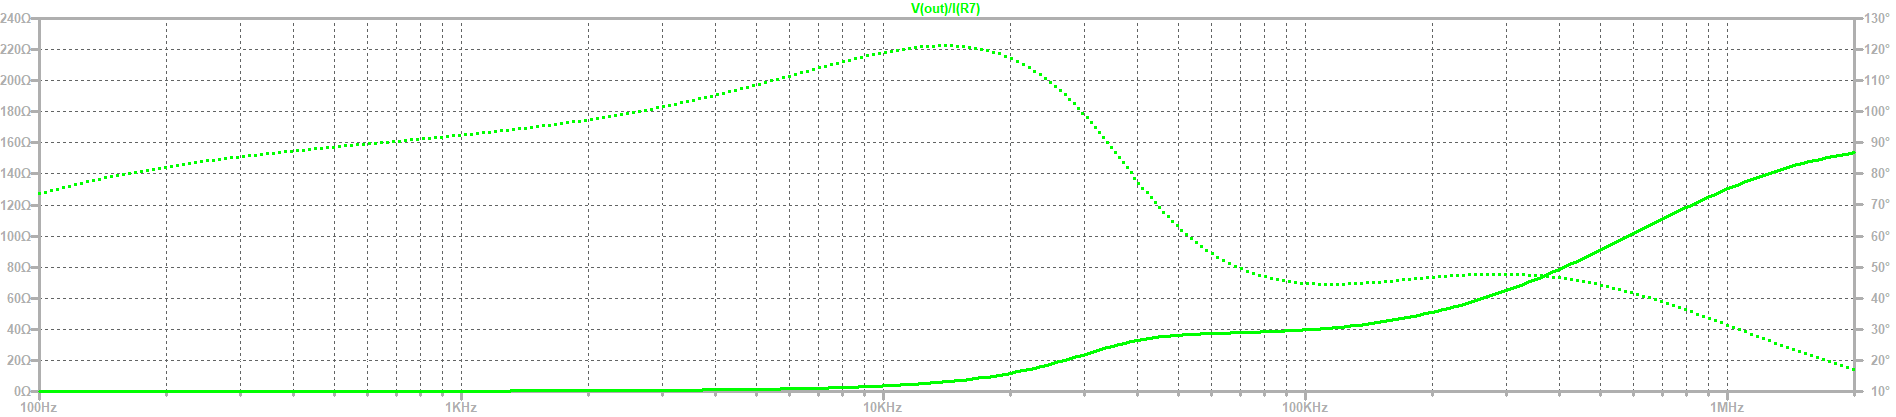
\includegraphics[width=\textwidth]{Imagenes-Ej2/ZoutE1.png}
	\label{fig:graph}
	\caption{Impedancia de salida 1er etapa.}
\end{figure}


\begin{figure}[H]
	\centering
	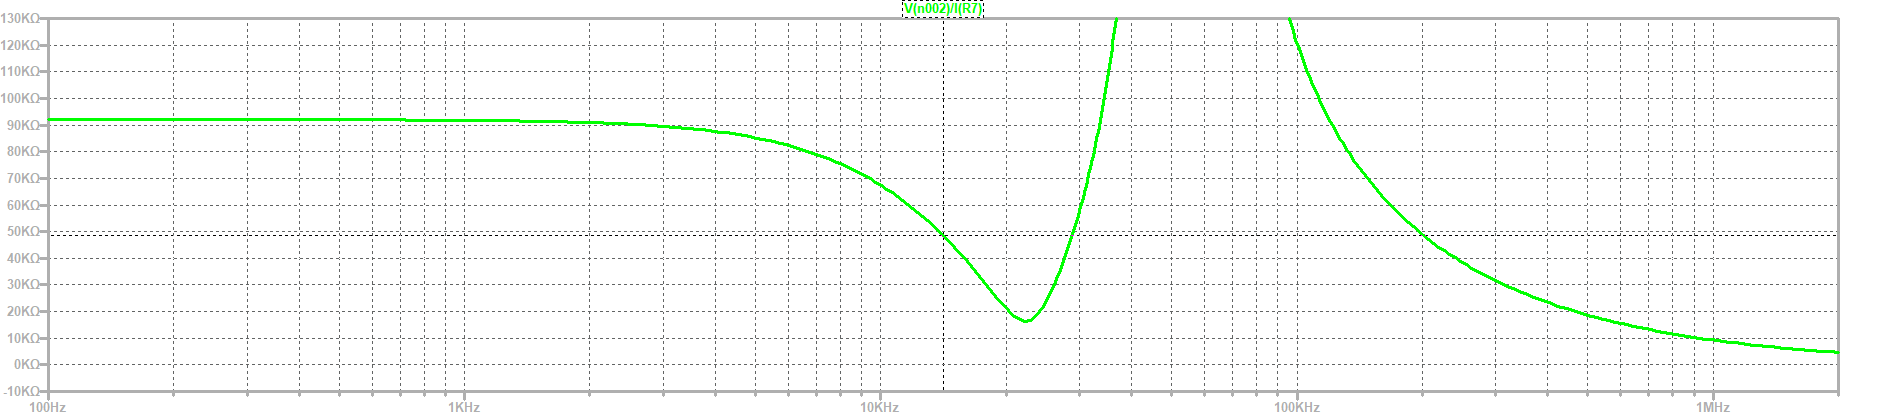
\includegraphics[width=\textwidth]{Imagenes-Ej2/ZinE2.png}
	\label{fig:graph}
	\caption{Impedancia de entrada 2da etapa.}
\end{figure}

\subsection{Respuesta en Frecuencia.}
Se realizó un análisis de Montecarlo a la respuesta en frecuencia del circuito, utilizando una tolerancia de las resistencias al 1$\%$ y capacitores al 10$\%$ obteniendo la siguiente disperción.
%\begin{figure}[H]
%	\centering
%	\includegraphics[width=0.4\textwidth]{/ImagenesEjercicio3/Graph.png}
%	\label{fig:graph}
%\end{figure}
También se midió la respuesta en frecuencia del filtro y se cotejó con la simulación.
\begin{figure}[H]
	\centering
	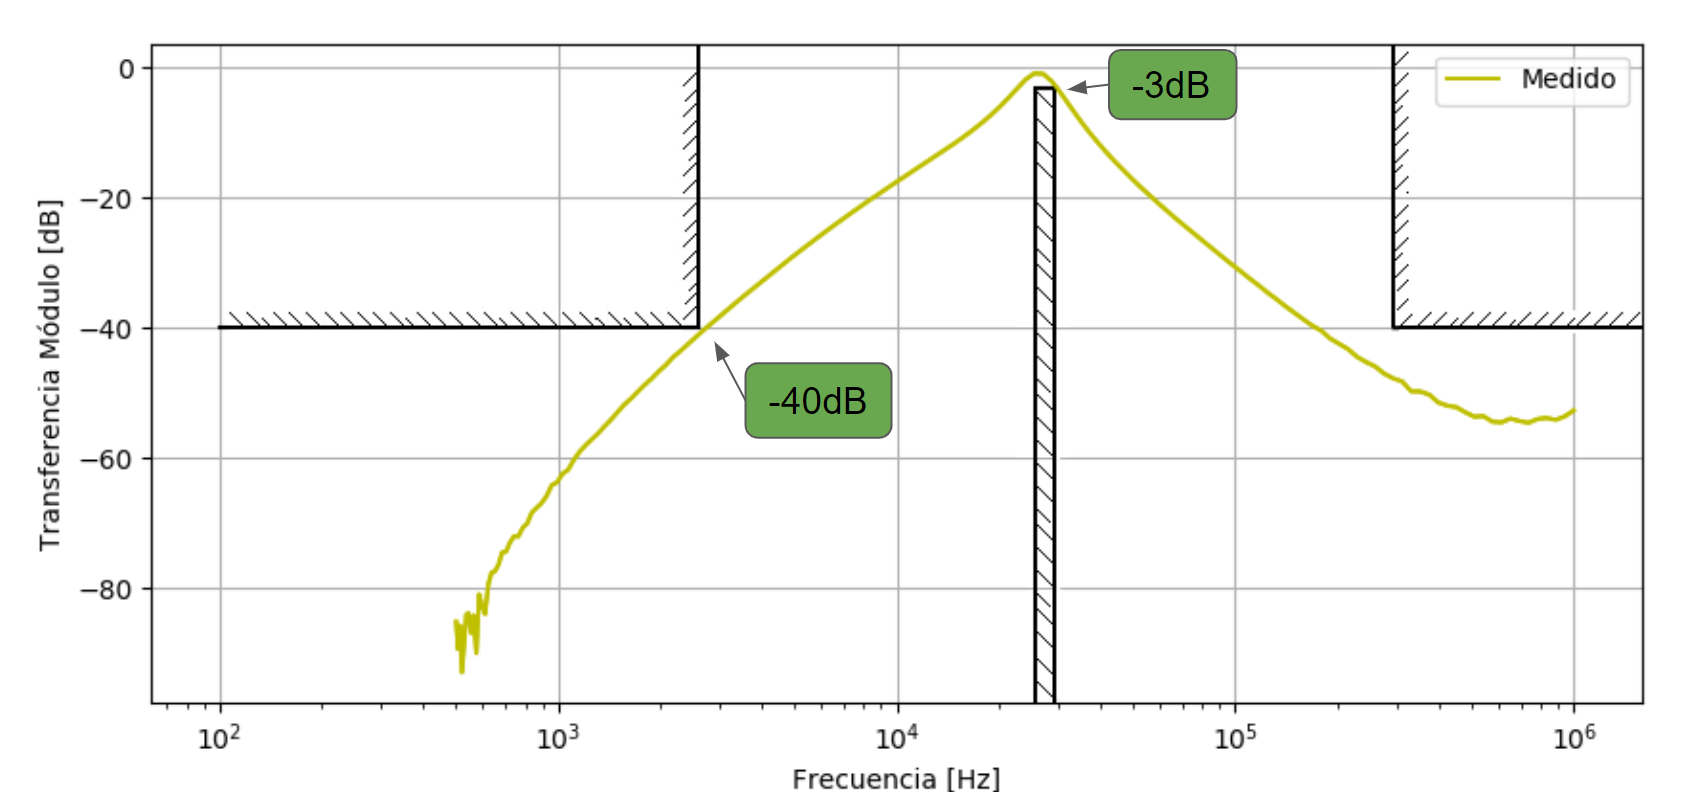
\includegraphics[width=\textwidth]{Imagenes-Ej2/BodeRauch.png}
	\label{fig:graph}
\end{figure}
\begin{figure}[H]
	\centering
	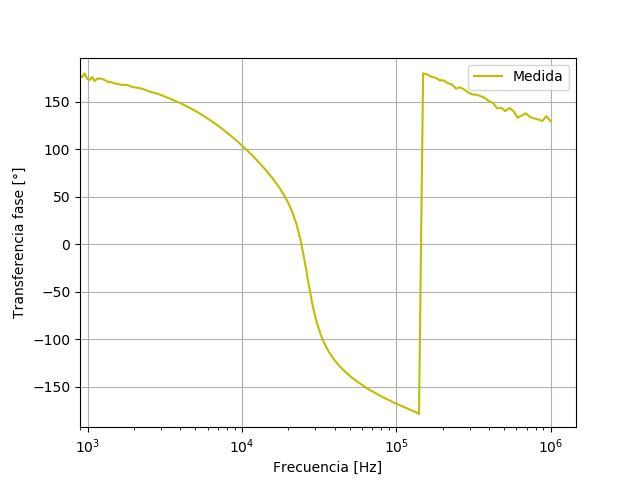
\includegraphics[width=\textwidth]{Imagenes-Ej2/BodeRauchFase.png}
	\label{fig:graph}
\end{figure}

\subsubsection{Etapas.}
Se realizaron 2 etapas, ambas siendo el mismo tipo de celda, pero con distintos parámetros.
\subsubsection{Filtro definitivo.}
%
%\begin{figure}[H]
%	\centering
%	\includegraphics[width=0.4\textwidth]{/ImagenesEjercicio3/Graph.png}
%	\label{fig:graph}
%\end{figure}

\end{document}
	\newpage
	
\section{Amplificadores de Instrumentación}
	\label{seccion:3}
	%\documentclass[a4paper]{article}
%\usepackage[spanish]{babel}
%\usepackage[utf8]{inputenc}
%\usepackage{float}
%\usepackage{graphicx}
%\usepackage[american voltage]{circuitikz}
%\usepackage{amsmath}
%\usepackage{xcolor}
%\usepackage{caption}
%\usepackage{subcaption}
%\usepackage[bottom]{footmisc}
\documentclass[a4paper]{article}
\usepackage[utf8]{inputenc}
\usepackage[spanish, es-tabla, es-noshorthands]{babel}
\usepackage[table,xcdraw]{xcolor}
\usepackage[a4paper, footnotesep = 1cm, width=20cm, top=2.5cm, height=25cm, textwidth=18cm, textheight=25cm]{geometry}
%\geometry{showframe}

\usepackage{tikz}
\usepackage{amsmath}
\usepackage{amsfonts}
\usepackage{amssymb}
\usepackage{float}
\usepackage{graphicx}
\usepackage{caption}
\usepackage{subcaption}
\usepackage{multicol}
\usepackage{multirow}
\setlength{\doublerulesep}{\arrayrulewidth}
\usepackage{booktabs}

\usepackage{hyperref}
\hypersetup{
    colorlinks=true,
    linkcolor=blue,
    filecolor=magenta,      
    urlcolor=blue,
    citecolor=blue,    
}

\newcommand{\quotes}[1]{``#1''}
\usepackage{array}
\newcolumntype{C}[1]{>{\centering\let\newline\\\arraybackslash\hspace{0pt}}m{#1}}
\usepackage[american]{circuitikz}
\usetikzlibrary{calc}
\usepackage{fancyhdr}
\usepackage{units} 

\graphicspath{{../Ejercicio-1/}{../Ejercicio-2/}{../Ejercicio-3/}{../Ejercicio-4/}}

\pagestyle{fancy}
\fancyhf{}
\lhead{22.01 Teoría de Circuitos}
\rhead{Mechoulam, Lambertucci, Rodriguez Turco, Londero, Galdeman}
\rfoot{\centering \thepage}

	\subsection{Introducción}
	Los amplificadores de instrumentación, también conocidos como \textbf{IN-AMP},  son utilizados para amplificar con alta precisión las señales provenientes de diversas unidades de adquisición de datos que no poseen la amplitud suficiente o estan demasiado contaminadas por ruido externo como para poder ser aprovechadas.
	\subsubsection{Diferencias entre \textbf{IN-AMP} y \textbf{OP AMP}}
	A simple vista un \textbf{IN-AMP} puede ser fácilmente confundido con un \textbf{OP AMP} dado que tiene varios rasgos en común. En primer lugar ambos dispositivos amplifican una señal diferencial, es decir que multiplican por un cierto factor la diferencia de potencial entre sus terminales de entrada. Por otro lado también poseen una elevada impedancia de entrada (del orden de los Megaohms) y una muy baja impedancia de salida de unos pocos ohms.
	No obstante, podemos notar algunas diferencias fundamentales entre ambos. Por ejemplo, para configurar la ganancia a lazo cerrado de un amplificador operacional se debe ajustar mediante resistores de retro-alimentación externos mientras que en un amplificador de instrumentación la ganancia puede venir predefinida por el fabricante o ajustada mediante una única \textbf{resistencia externa} denominada usualmente como \textbf{$R_{gain}$}.
	En caso de que se desee amplificar una señal diferencial el amplificador de instrumentación eliminara cualquier componente de señal común a ambas entradas como puede ser un offset de continua o simplemente ruido. Esta característica es la que hace especiales a los amplificadores de instrumentación ya que permiten reducir de manera significativa el ruido de las señales recibidas.  
	Por el contrario, los amplificadores operacionales tradicionales que no están diseñados para eliminar este tipo señales no deseadas.

	
	\subsection{Características del IN-AMP}
	El circuito a analizar es una variante de los famosos amplificadores de instrumentación que utilizan 3 amplificadores operacionales que se puede observar en la figura debajo.
	%Imagen del amplificador de instrumentación con 3 op-amps
	\begin{figure}[H]
		\centering		
		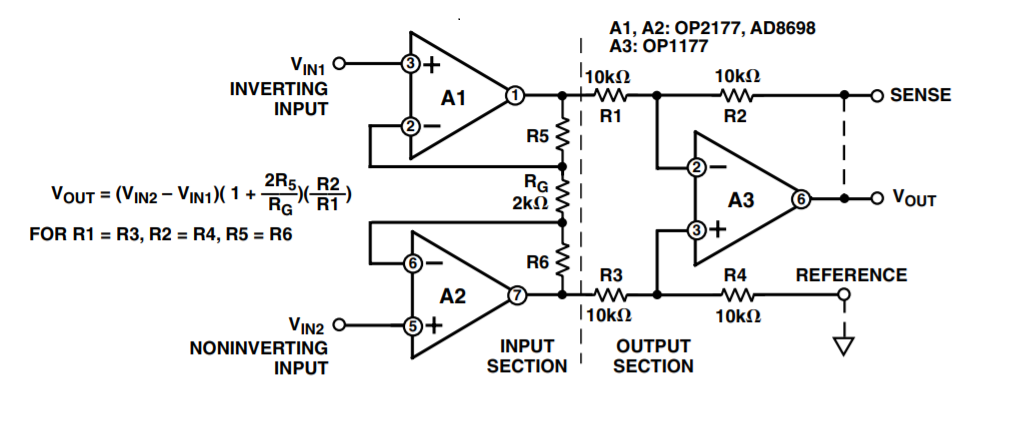
\includegraphics[width=\linewidth]{./ImagenesVarias/inAmp3Opamp}
		%TODO revisar footnote imagen 
		\caption{Clásico amplificador de instrumentación con 3 Opamps}
	\end{figure}
	%\footnote{Imagen extraída de: \textit{A designer's guide to Sinstrumentation amplifiers}
		
	Como se puede apreciar a la izquierda de la línea punteada se han colocado un par de buffers con ganancia. El objetivo de los mismos es de el de aumentar significativamente la impedancia de entrada del in-amp para independizarla lo más posible de la impedancias de las fuentes ya que este pueden ser muy altas o estar desbalanceadas. También ofrece la ventaja de no cargar a la fuente, lo cual es de gran relevancia al trabajar con señales pequeñas. Además le otorga una cierta ganancia a la señal de entrada. Este aspecto del circuito se debe tener en cuenta para evitar la saturación de los op-amps y perder la efectividad del circuito. Analizaremos esta y otras situaciones en secciones posteriores.
	En nuestro caso se trabajara con la versión de 4 amplificadores operacionales.
	
	\begin{figure}[H]
		\centering
		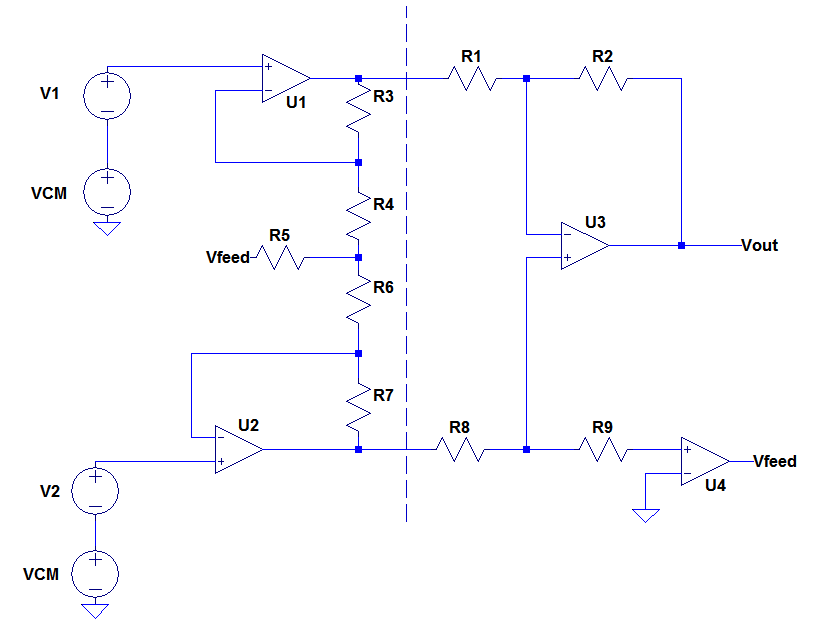
\includegraphics[width=\linewidth]{./ImagenesVarias/inAmpSch.png}
		\caption{Amplificador de instrumentación de 4 op-amps}
	\end{figure}

	Haciendo uso de la herramienta de análisis simbólico \textit{SapWin \footnote{SapWin es una programa de análisis y simulación de circuitos desarrollado por la \textit{Universitá degli studi Firenze}}} obtenemos la siguiente expresión para la ganancia ideal de amplificador de instrumentación:
	\begin{equation}
			V_{out}=\frac{-V_1 R_2 R_4 R_7 - 
			V_1 R_2 R_3 R_7 +
			V_2 R_2 R_3 R_7+
			V_2 R_2 R_3 R_6
		}{R_1 R_4 R_7}
		\label{eqn:idealTrans}
	\end{equation}

	
	Notamos que en la situación ideal tanto las resistencias $R_5$ y $R_9$ no afectan la ganancia del circuito.
	\subsubsection{Relaciones entre los componentes}
	Una de las finalidades del amplificador de instrumentación es la de eliminar aquellas señales que sean comunes a las señales de entrada.
	Por tal motivo comenzaremos por establecer condiciones que nos permitan eliminarlas. 
	Para eso aplicaremos superposición y analizaremos los efectos de $V_{CM}$ sobre la relación anterior.
	
	\begin{figure}[H]
		\centering
		\includegraphics[width=\linewidth]{./ImagenesVarias/inAmpVCM.png}
		\caption{Amplificador de instrumentación de 4 op-amps en modo común}
	\end{figure}
	Obteniendo como transferencia:
	\begin{equation}
		\frac{V_{out}}{V_{CM}}=
		\frac{-R_2 R_4 R_7 - 
			R_2 R_3 R_7 +
			R_2 R_3 R_7+
			R_2 R_3 R_6
		}{R_1 R_4 R_7}
	\end{equation}
		
	Como se quiere que aquellas señales comunes a ambas entrada sean eliminadas pedimos $V_{out}=0$.
	Entonces obtenemos:
		\begin{equation}
		 0=\frac{-V_{CM} R_2 R_4 R_7 - 
				V_{CM} R_2 R_3 R_7 +
				V_{CM} R_2 R_3 R_7+
				V_{CM} R_2 R_3 R_6
			}{R_1 R_4 R_7} 
		\end{equation}
	
	Simplificando
	\begin{equation}
		R_7(R_4+R_3)=R3(R7+R6)
	\end{equation}
	
	\begin{equation}
		R_7R_4+ R_3R_7=R_3R_7+R_3R_6
	\end{equation}
	Cancelando los términos comunes a ambos miembros
	\begin{equation}
		R_7R_4=R_3R_6
	\end{equation}
	Por lo tanto llegamos a:
	\begin{equation}
		\frac{R_4}{R_6}=\frac{R_3}{R_7}  %Relación entre las resistencias de la etapa de amplificación
	\end{equation}

	Aplicando estas relaciones a \eqref{eqn:idealTrans} obtenemos:
	\begin{equation}
		V_{out} = (V_2-V_1)\left[\frac{R_2}{R_1}(1+\frac{R_3}{R_4})\right]
	\end{equation}
En nuestro afán de conseguir una amplificación de 137,32 se realizaron las siguientes consideraciones en busca de conseguir la configuración más simétrica posible.
En primer lugar dadas las limitaciones de las tolerancias de los componentes se decidió implementar un amplificador de instrumentación con una ganancia de 137,5 veces. Sí bien se podría haber intentado calibrar la ganancia del mismo mediante el uso de resistores variables, debemos tener en cuenta que los presets no son ajustables con la suficiente precisión y estos además cuentan con su correspondiente tolerancia. Por otro lado a causa de vibraciones o movimientos bruscos los mismos podrían cambiar su valor forzando al usuario a chequear sus valores previo al uso. 
En segundo lugar se eligieron que las resistencias $R_3$ y  $R_4$ tomasen el mismo valor. Este decisión obligara a que $R_7$ y  $R_6$ también sean iguales. Por lo tanto conseguimos mucha simetría en la primera etapa

\begin{equation}
	V_{out} = (V_2-V_1)\left[2 \frac{R_2}{R_1}\right]
\end{equation}

Luego se eligió $R_2$ del mismo orden de magnitud que $R_1$ de forma tal que el factor de \textbf{2} que apareció previamente sea cancelado y $R_2$ controle por completo la ganancia. Esta $R_2$ fue armada mediante 2 resistores SMD en serie.

\begin{table}[H]
	\centering
	\begin{tabular}{lll}
		Componente  & Valor        	   & Tolerancia \\
		\\
		$R_1$       & 2K$\Omega$   	   & 1\%        \\
		$R_2$       & 130K$\Omega$ 	   & 1\%        \\
		$R_{2'}$  	& 7,5K$\Omega$     & 1\%        \\
		$R_3$ 		& 10K$\Omega$      & 1\%		\\
		$R_4$		& 10K$\Omega$      & 1\%        \\
	    $R_5$		& 10K$\Omega$      & 1\%        \\
	    $R_6$		& 10K$\Omega$      & 1\%        \\
	    $R_7$		& 10K$\Omega$      & 1\%        \\
	    $R_8$		& 2K$\Omega$       & 1\%        \\
 	    $R_9$		& 130K$\Omega$     & 1\%        \\   
		$R_{9'}$	& 7,5K$\Omega$     & 1\%        \\
			\end{tabular}
		\caption{Tabla de valores de componentes del IN-AMP al 1\%}
\end{table}

\begin{figure}[H]
	\centering
	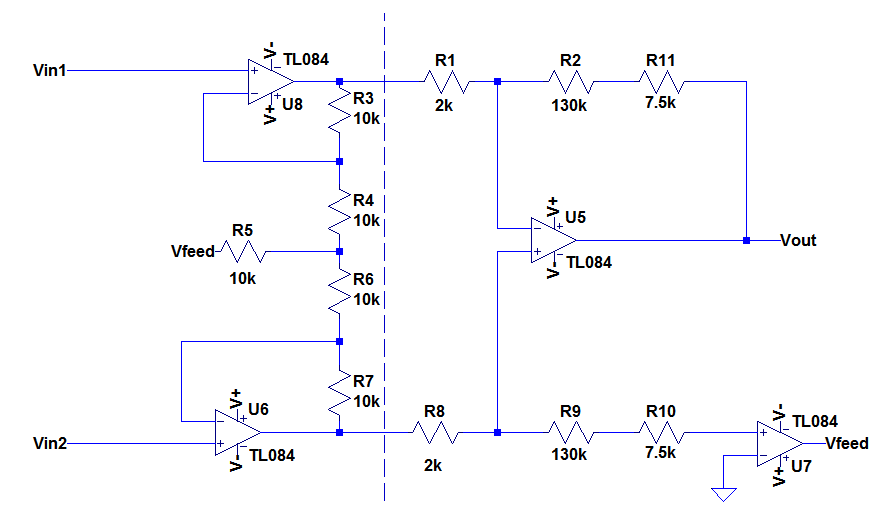
\includegraphics[width=\linewidth]{./ImagenesVarias/IN-AMP-CON-VALORES.png}
	\caption{IN-AMP con los valores elegidos}
\end{figure}

  Cabe destacar que el orden de magnitud de los componentes se baso en que los amplificadores de instrumentación comerciales son fabricados con resistencias en el orden de los K-ohms.
  
  Como fue antes mencionado, el amplificador de instrumentación debe poseer, idealmente, impedancia de entrada infinita. Para poder aproximarnos lo más posible a este ideal se decidió utilizar el amplificador operacional \textbf{TL084} que posee una impedancia de entrada de 1 Tera-Ohm ($10^{12}\Omega$). Otra ventaja de elegir este operacional es que se consiguen en un solo integrado que contiene a los de 4 op-amps dentro de un mismo integrado lo cual disminuye las variaciones por cambios de temperatura dado que se encuentran los 4 bajo las mismas condiciones de operación.
  
\subsection{Efecto de las tolerancias}
Cuando se plantearon los primeros amplificadores diferenciales se utilizaron configuraciones simples como la exhibida debajo, ya se conocía que los resistores $R_1$, $R_2$, $R_3$ y $R_4$ debían estar apropiadamente balanceados con el fin de maximizar el rechazo en modo común. 
\begin{figure}[H]
	\centering
	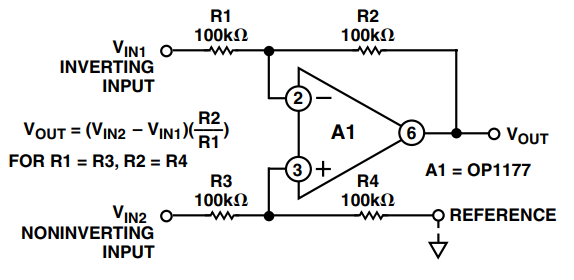
\includegraphics[width=\linewidth]{./ImagenesVarias/AmplificadorDiferencial.PNG}
	\caption{Amplificador diferencial}
\end{figure}  

Sin embargo las tolerancias de los componentes no lo permiten. Es por tal motivo que para alcanzar dicha precisión los fabricantes construyen dichas resistencias, mediante técnicas láser durante el proceso de fabricación del IC con el fin de minimizar esas diferencias.

El modelo más sofisticado y robusto que se implemento presenta mejoras muy notables por sobre su antecesor. No obstante, estas mejoras también traen nuevos desafíos dado que se añaden más componentes resistivos al sistema.

Usando resistencias al 1\% obtenemos la siguiente simulación de Montecarlo para en modo diferencial

\begin{figure}[H]
	\centering
	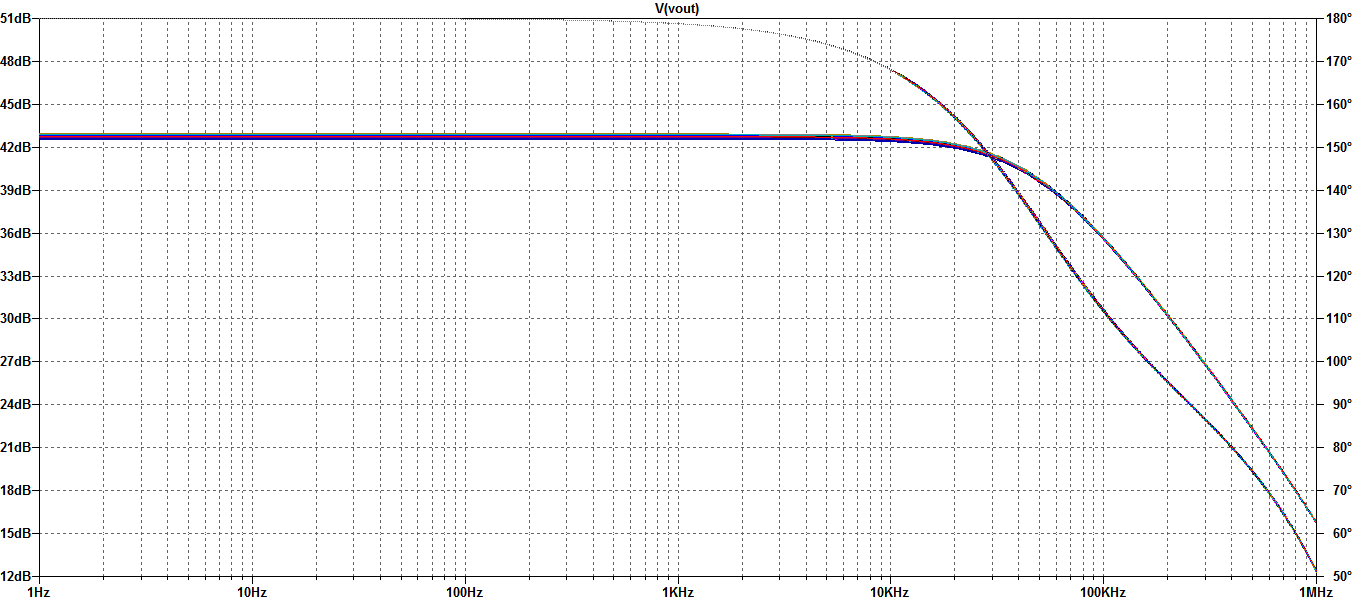
\includegraphics[width=\textwidth]{./ImagenesDeSimulaciones/MonteCarloModoDiferencialGrande.png}
	\caption{Montecarlo en modo diferencial}
\end{figure}  
Como podemos notar, las tolerancias no afectan significativamente su desempeño en modo diferencial.

Sin embargo podemos realizar más observaciones en cuanto a su desempeño en modo comúm
\begin{figure}[H]
	\centering
	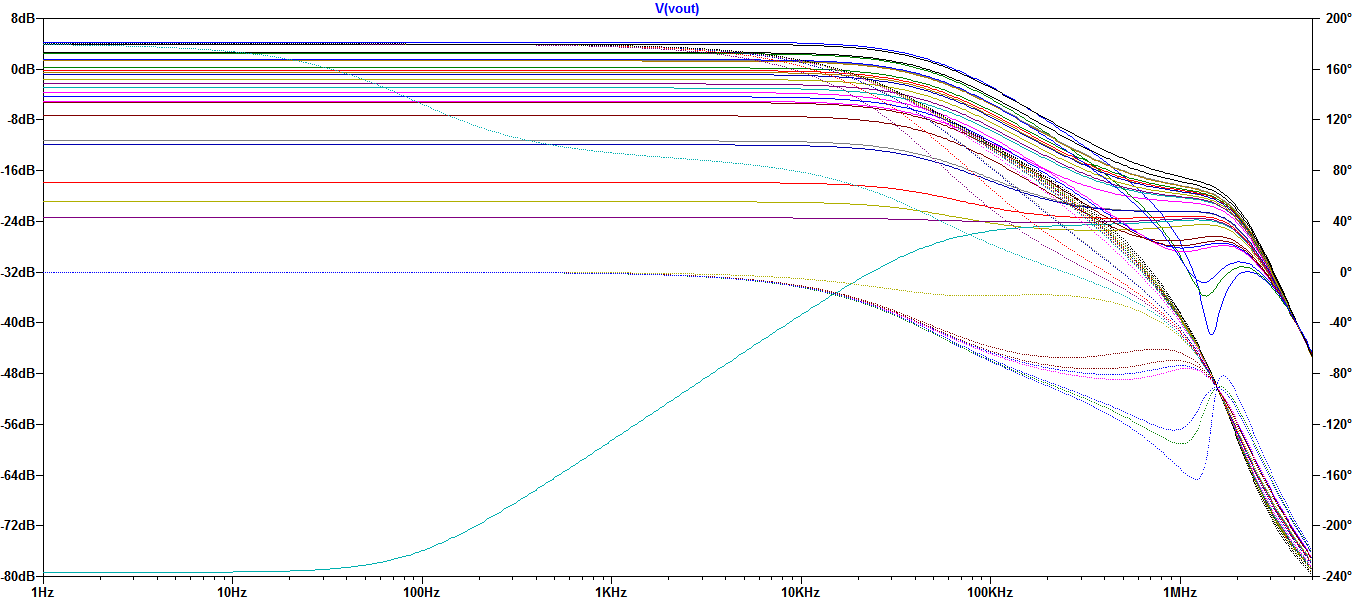
\includegraphics[height=0.3\textheight]{./ImagenesDeSimulaciones/MonteCarloModoComunGrande1V.png}
	\caption{Montecarlo en modo común con 1 Vpp de entrada}
\end{figure} 
Este gráfico de bode pone en evidencia la importancia de que las resistencias poseean la mayor precisión posible.

Si la tensión en modo común se reduce vemos como mejora el rechazo en modo común.
\begin{figure}[H]
	\centering
	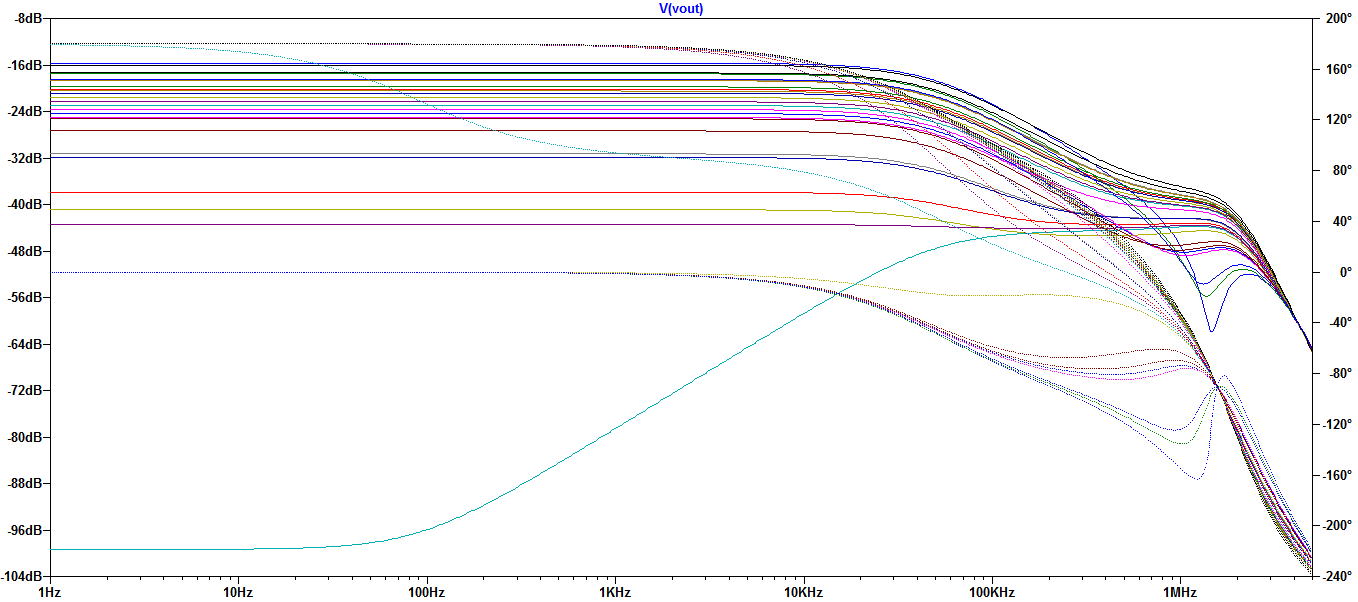
\includegraphics[height=0.3\textheight]{./ImagenesDeSimulaciones/MonteCarloModoComunGrande100mv.png}
	\caption{Montecarlo en modo común con 100 mv de entrada}
\end{figure} 

También se intento ver los alcances de rechazo común frente a una continua
\begin{figure}[H]
	\centering
	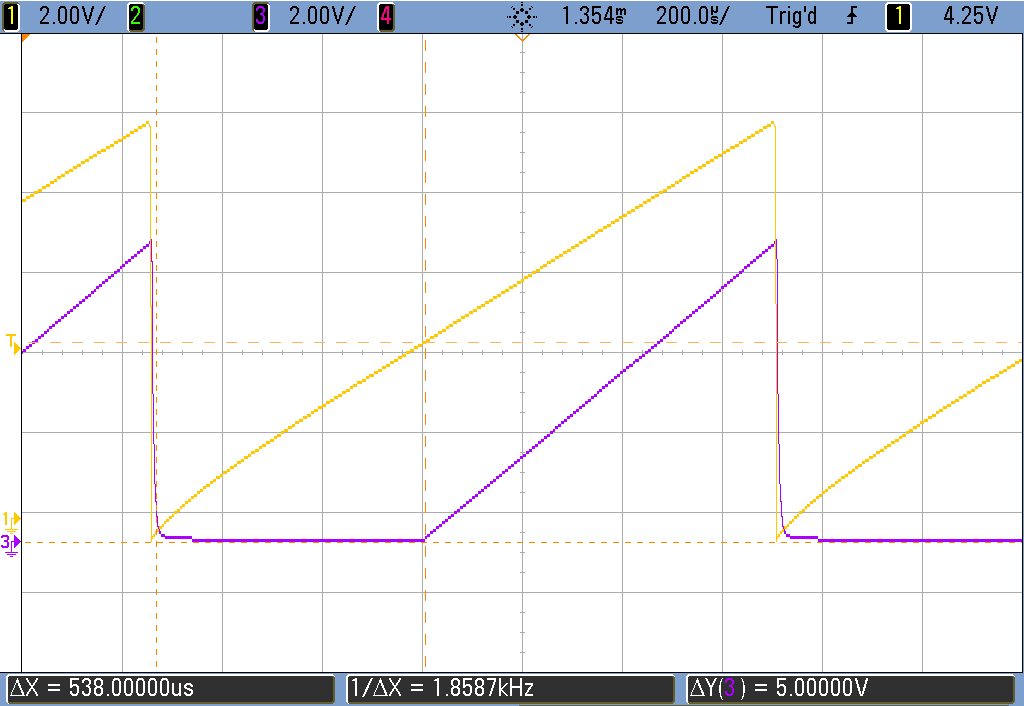
\includegraphics[height=0.3\textheight]{./ImagenesDeOsciloscopio/ModoComunContinua.png}
	\caption{Rampa de 0 a 20V}
\end{figure} 

Vemos como el circuito es capaz de soportar hasta unos 5V de continua (como indica el cursor) antes de salir de su zona de operación.

\subsection{Respuesta en frecuencia}
Los amplificadores de instrumentación obtienen su mejor rendimiento en la rango de las frecuencias medias a bajas. Esta configuración exhibe un comportamiento del tipo pasabajos lo que provoca que no se obtenga la ganancia esperada a frecuencias elevadas.
\begin{figure}[H]
	\centering
	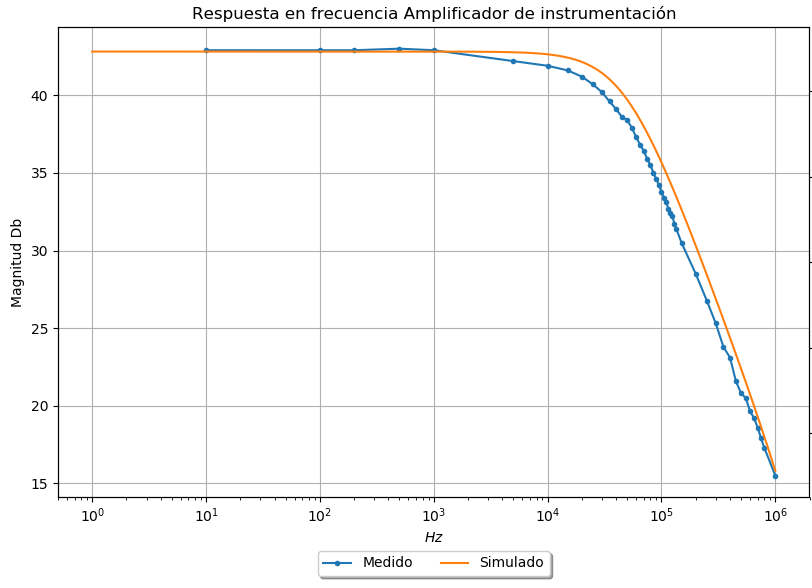
\includegraphics[height=0.3\textheight]{./ImagenesVarias/BODE_MAG.PNG}
	\caption{Bode de Magnitud}
\end{figure}


  
  
  
  
  
  
  
  
  
  
  
  
  
  
  
  
  
\subsection{Generación de señales con puente de Wheatstone}
Se diseño un puente de WheatStone para la generación de señales compuestas.
\begin{figure}[H]
	\centering
	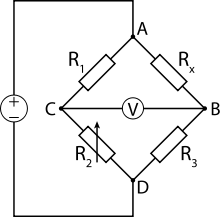
\includegraphics[height=0.25\textheight]{./ImagenesVarias/wheatstone.png}
	\caption{Puente de WheatStone}
\end{figure}

Este método emula a un sensor que utilice un sistema tipo puente con un resistor variable que puede llegar a cambiar de valor según la temperatura, presión u alguna otra que ocasiona que su valor cambie.

\begin{figure}[H]
	\centering
	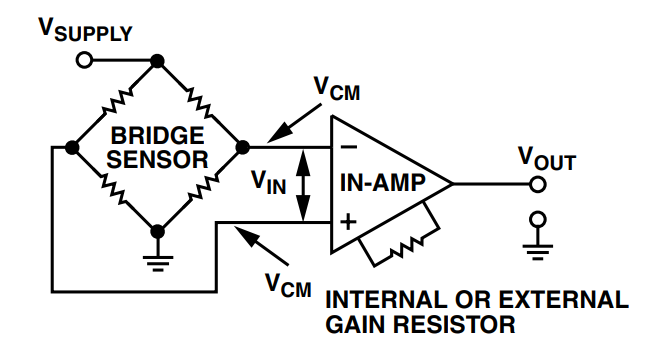
\includegraphics[height=0.3\textheight]{./ImagenesVarias/wheatstoneInAmp.png}
	\caption{IN-AMP con puente de WheatStone Acoplado}
\end{figure}

La tensión suministrada en la parte superior del puente permite que las variaciones de resistencia se traduzcan en una señal eléctrica.
Sin embargo es necesario poseer una cierta referencia para poder determinar si de hecho ocurrió un cambio. Es por es que el amplificador de instrumentación se vale del puente y de sus 2 bornes de salida para llevar acabo esta detección. La rama del puente que cuenta con sus resistores fijos proporcionara la tensión de referencia.
A la entrada del amplificador de instrumentación se le proporcionaran 2 señales. En primer tendremos la señal de referencia y por el otro la señal portadora de la perturbación.
Debemos notar que dado el diseño del amplificador de instrumentación de no haber diferencias entre las dos señales entonces en el caso ideal se debería observar una salida nula. 

Para el armado del puente se eligieron resistores con tolerancias del 1\% para mantener el puente lo más balanceado posible y maximizar el rechazo en modo común.
\begin{table}[H]
	\centering
	\begin{tabular}{lll}
		Componente  		& Valor        	& Tolerancia \\
		\\
		$R_1$       		& 10K$\Omega$   & 1\%        \\
		$R_2$       		& 10K$\Omega$ 	& 1\%        \\
		$R_{2'}$ Preset      & 1K$\Omega$ 	& 10\%        \\
		$R_3$  				& 10K$\Omega$   & 1\%        \\
		$R_4$ 				& 10K$\Omega$   & 1\%		\\
	\end{tabular}
	\caption{Tabla de valores de componentes del puente de WheatStone al 1\%}
\end{table}

El preset nos permite generar de manera artificial "la perturbación" sobre la señal.

\begin{figure}[H]
	\centering
	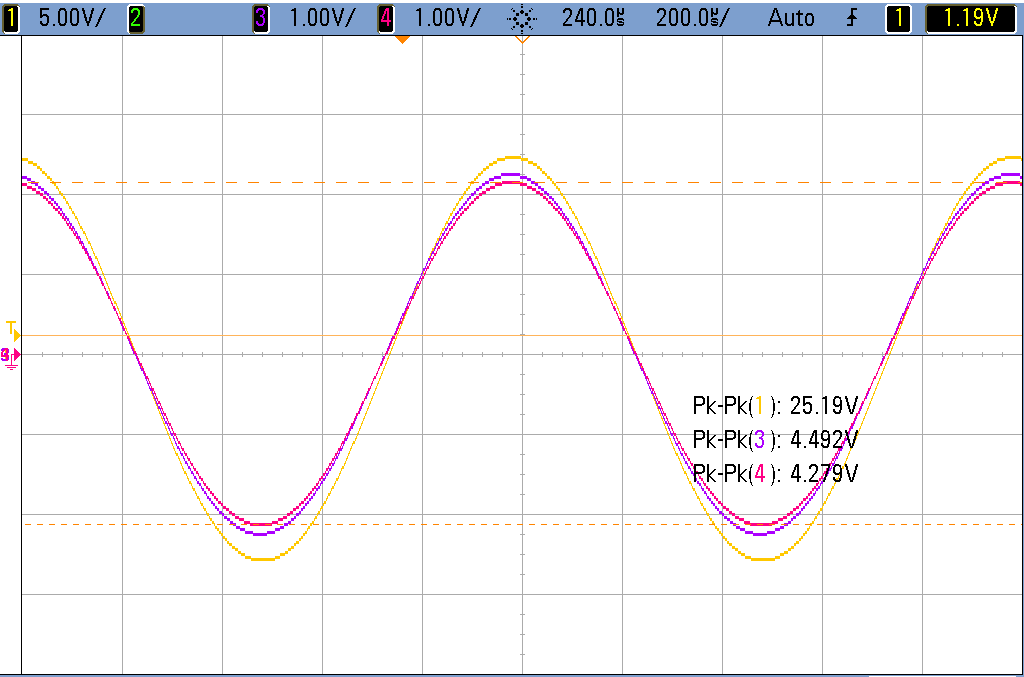
\includegraphics[height=0.3\textheight]{./ImagenesDeOsciloscopio/WheatStone1tierra1c1R.png}
	\caption{Amplificación de diferencias con puente de WheatStone}
\end{figure}
Notese la escala de las señales.
\subsubsection{Análisis de Tolerancias en el puente de WheatStone}


\subsubsection{Señales con y sin referencia a tierra}
La problemática al medir señales con entrada flotante, como pueden ser por ejemplo los transformadores o cualquier otro señal que se encuentre aislada de tierra radica en el hecho que las corrientes de bias del amplificador de instrumentación, no tanto las inherentes al dispositivo por cuestiones de fabricación, sino más bien aquellas desarrolladas por el aumento de la temperatura. Es de mayor relevancia en los \textbf{IN-AMP} desarrollados con transistores \textbf{FET} que, aunque tiene menores corrientes de bias a temperatura ambiente, estas se duplican cada 11 grados centigrados. Estas corrientes provocan que el amplificador de instrumentación conmute más rápidamente observándose cierto "ruido" en la señal de salida. Se recomienda siempre colocar un camino entre la fuente flotante y ground. Esto se puede lograr utilizando un resistor de entre $1M\Omega$ y  $10\Omega$

\begin{figure}[H]
	\centering
	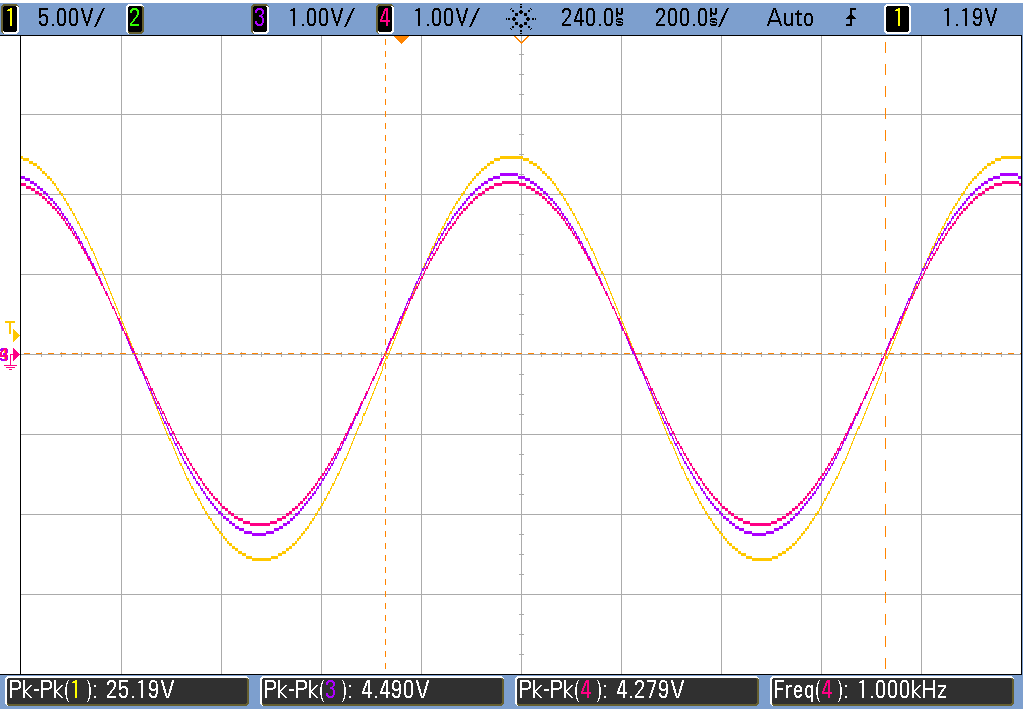
\includegraphics[height=0.3\textheight]{./ImagenesDeOsciloscopio/WheatStoneTierra1.png}
	\caption{Amplificación de diferencias con puente de WheatStone con conexión a ground}
\end{figure}

\begin{figure}[H]
	\centering
	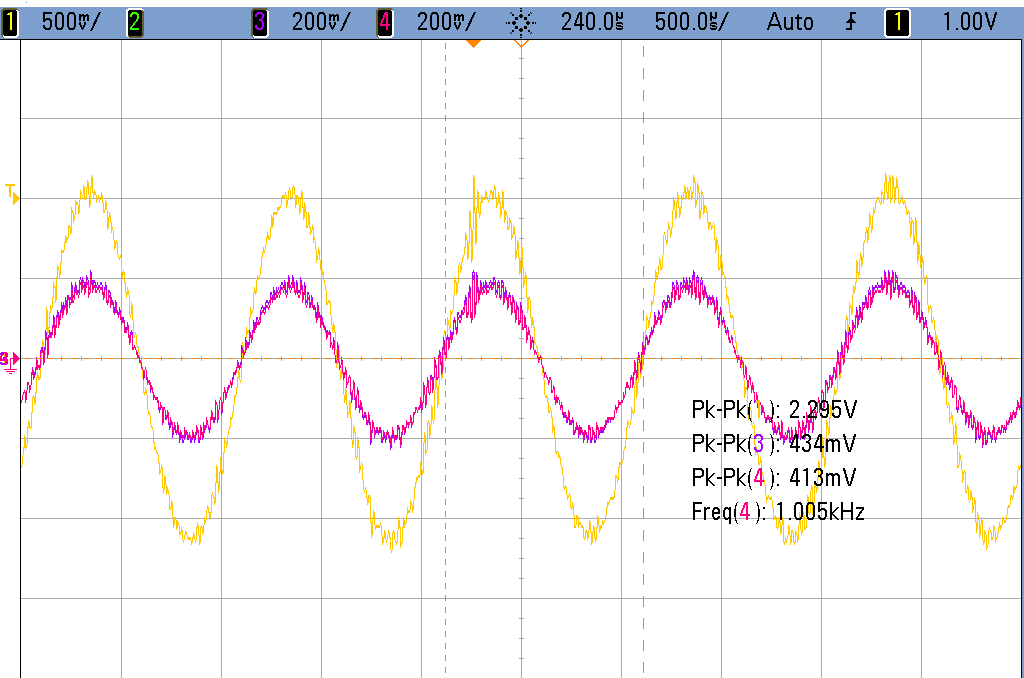
\includegraphics[height=0.3\textheight]{./ImagenesDeOsciloscopio/WheatstoneAislado.png}
	\caption{Amplificación de diferencias con puente de WheatStone con conexión a ground}
\end{figure}




 	
\begin{thebibliography}{9}
	
	\bibitem{Franco} 
	SERGIO, F. (2002). Design with operational amplifiers and analog integrated circuits. New York [etc.]: McGraw-Hill, pp.73-91.	
	
	\bibitem{Coughlin} 
	R. Coughlin and F. Driscoll, Circuitos integrados lineales y amplificadores operacionales. México: Prentice-Hall Hispanoamericana, 1998.
	
	\bibitem{dguideinamp}
	C. Kitchin and L. Counts, A designer's guide to instrumentation amplifiers. Norwood, Mass.: Analog Devices, 2006.
	
	\bibitem{an244}
	Jeffrey R. Riskin, A User's guide to IC instrumentation amplifiers. Norwood, Mass.: Analog Devices.
	
\end{thebibliography}

	\newpage

\section{Circuito de Medicion de Presion}
	\documentclass[a4paper]{article}
\usepackage[spanish]{babel}
%Para uso de palabras acentuadas
\usepackage[utf8]{inputenc}

\documentclass[a4paper]{article}
\usepackage[utf8]{inputenc}
\usepackage[spanish, es-tabla, es-noshorthands]{babel}
\usepackage[table,xcdraw]{xcolor}
\usepackage[a4paper, footnotesep = 1cm, width=20cm, top=2.5cm, height=25cm, textwidth=18cm, textheight=25cm]{geometry}
%\geometry{showframe}

\usepackage{tikz}
\usepackage{amsmath}
\usepackage{amsfonts}
\usepackage{amssymb}
\usepackage{float}
\usepackage{graphicx}
\usepackage{caption}
\usepackage{subcaption}
\usepackage{multicol}
\usepackage{multirow}
\setlength{\doublerulesep}{\arrayrulewidth}
\usepackage{booktabs}

\usepackage{hyperref}
\hypersetup{
    colorlinks=true,
    linkcolor=blue,
    filecolor=magenta,      
    urlcolor=blue,
    citecolor=blue,    
}

\newcommand{\quotes}[1]{``#1''}
\usepackage{array}
\newcolumntype{C}[1]{>{\centering\let\newline\\\arraybackslash\hspace{0pt}}m{#1}}
\usepackage[american]{circuitikz}
\usetikzlibrary{calc}
\usepackage{fancyhdr}
\usepackage{units} 

\graphicspath{{../Ejercicio-1/}{../Ejercicio-2/}{../Ejercicio-3/}{../Ejercicio-4/}}

\pagestyle{fancy}
\fancyhf{}
\lhead{22.01 Teoría de Circuitos}
\rhead{Mechoulam, Lambertucci, Rodriguez Turco, Londero, Galdeman}
\rfoot{\centering \thepage}

\usepackage{float}
\usepackage{graphicx}

\usepackage[american voltage]{circuitikz}

\usepackage{amsmath}

\usepackage{xcolor}

\usepackage{caption}
\usepackage{subcaption}

\begin{document}

\section{Circuitos integradores y derivadores}
\subsection{Introducción}
Los circuitos implementados con amplificadores operacionales permiten la implementación de diferentes configuraciones que resuelven problemas matemáticos. Con el diseño adecuado pueden usarse para resolver sistemas de ecuaciones diferenciales.
En este caso estudiaremos 2 bloques fundamentales. El circuito integrador y el derivador. Se analizaran sus características más relevantes así como también sus límites de uso y como extenderlos para aprovecharlos al máximo.

\begin{figure}[hbt!]
	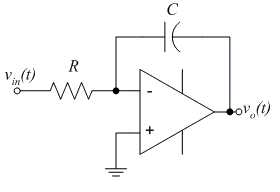
\includegraphics[scale=1]{Ejercicio4/integrador.png}
	\caption{Circuito integrador} 
	
	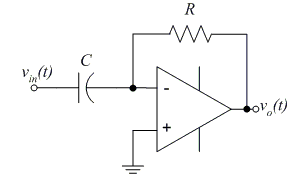
\includegraphics{Ejercicio4/derivador}
	\caption{Circuito Derivador} 
	
\end{figure}

\subsection{Análisis previo del \textbf{LM833N}}
El amplificador a utilizar es el \textbf{LM833N} de STMicroelectronics. El mismo es un operacional de bajo ruido diseñado para aplicaciones relacionadas al manejo de audio.
En su hoja de datos podemos ver que posee un alto nivel Slew Rate de hasta 7 $\frac{V}{s}$, un GBP de 15MHz y una ganancia de tensión 
a lazo abierto típica de unos 110 dB. Notemos que también se indica que la ganancia mínima es de unos 90 dB. 


 \subsubsection{Cálculo de $A_{vol}$}
Para poder realizar los cálculos de transferencia y establecer sus correspondientes transferencias de teóricas primero debemos conocer $A_{vol}$ medido en veces. Para esto basta con tomar el valor de ganancia de tensión típica a veces.
$$A_{vol} = 10^{\frac{110}{20}}$$
$$A_{vol} \approx 316.227,77$$

\subsubsection{Cálculo de  la $f_p$, polo dominante}

Dado el \textbf{GBP} de 15MHz podemos fácilmente calcular la frecuencia de corte a lazo abierto

$$ f_p = \frac{15MHz}{A_{vol}} $$
$$ f_p \approx 47.44Hz$$

\section{Ganancia bajo diferentes condiciones de $A_{vol}$}
En esta sección analizaremos las características de la ganancia de tensión brindad por ambos circuitos bajo diferentes condiciones.

\subsection{$A_{vol}$ infinito}
En un circuito con amplificadores operacionales es deseable utilizar dispositivos con $A_{vol}$(ganancia a lazo abierto) lo más alto posible para que los modelos teóricos se aproximen a su implementación física.

Ambos circuitos adoptan la configuración de un circuito inversor y sus transferencias pueden ser descritas mediante
$$H(s)_{inv} = \frac{-\frac{Z_{Feed}}{Z_{in}}}
{1+\frac{1+\frac{Z_{Feed}}{Z_{in}}}{A_{vol}}} $$
La cual representa la función transferencia de un amplificador operacional no ideal.
Si consideramos $A_{vol}$ infinito obtenemos la transferencia para el inversor ideal:
$$H(s)_{inv} = \frac{-\frac{Z_{Feed}}{Z_{in}}}
				{1+\underbrace{\frac{1+\frac{Z_{Feed}}{Z_{in}}}{A_{vol}}}_{\text{\shortstack{$A_{vol}\rightarrow \infty$ \\ $\rightarrow 0$}}}}$$

$$H(s)_{ideal} =  -\frac{Z_{Feed}}{Z_{in}}$$

Entonces para el circuito integrador obtenemos:
$$H(s)_{\int_{}{}} = \frac{-1}{sCR} $$

Podemos corroborar que la acción de este circuito es integrar la señal de entrada al realizar la transformada inversa de Laplace
$$v_{out}(t) = \mathcal{L}^{-1}[X(s)H(s)_{\int_{}{}}]$$
$$v_{out}(t) = \mathcal{L}^{-1}[X(s)\cdot \frac{-1}{sCR}]$$
$$v_{out}(t)= \frac{-1}{CR} \cdot \int_{0}^{t}v_t dt$$            
\\
Por otro lado tenemos el circuito derivador:
$$H(s)_{\frac{d}{dt}}=-sCR$$
Análogamente aplicamos la anti-transformada de Laplace:

$$v_{out}(t) = \mathcal{L}^{-1}[X(s)H(s)_{\frac{d}{dt}}]$$

$$v_{out}(t) = \mathcal{L}^{-1}[X(s)\cdot (-sCR)]$$

$$v_{out}(t)= -CR \frac{d}{dt}v_t(t)$$       

Si bien, estos circuitos tienen la capacidad de realizar las operaciones antes mencionadas, en los párrafos siguientes estudiaremos su comportamiento y bajo que condiciones funcionan.

\subsubsection{Diagramas de Bode con $A_{vol}$ ideal}
\begin{figure}[H]
	\centering
	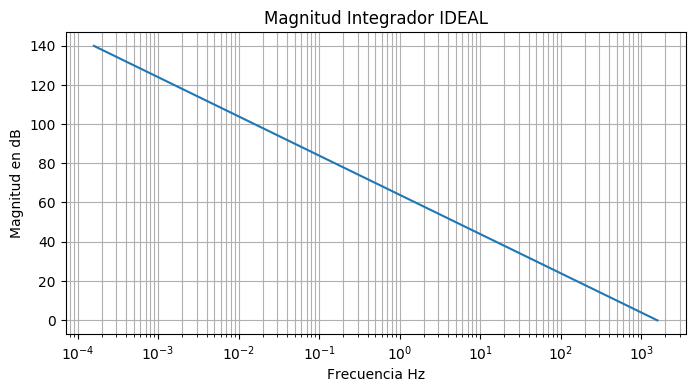
\includegraphics[width=\textwidth]{Ejercicio4/BODE-IDEAL-MAGNITUD-INTEGRADOR.png}
	\caption{Ganancia Ideal Circuito Integrador}
\end{figure}

Observamos que el integrador ideal tiene una muy alta ganancia a bajas frecuencias y muy baja cuando se acerca a los $10KHz$ lo cual limita su rango de operación.

\begin{figure}[H]
	\centering
	\includegraphics[width=\textwidth]{Ejercicio4/BODE-IDEAL-MAGNITUD-DERIVADOR.png}
	\caption{Ganancia Ideal Circuito Derivador}
\end{figure}
De modo contrario el derivador exhibe sus capacidades a altas frecuencias
\\*
En cuanto a la fase en ambos casos podemos observar como ver cómo las operaciones de integración y diferenciación introducen un desfase de $\pm90^{\circ}$ de la señal original según el caso. 
\begin{figure}[H]
	\centering
	\includegraphics[width=\textwidth]{Ejercicio4/BODE-IDEAL-FASE-INTEGRADOR.png}
	\caption{Fase Ideal Circuito Integrador}
\end{figure}

\begin{figure}[H]
	\includegraphics[width=\textwidth]{Ejercicio4/BODE-IDEAL-FASE-DERIVADOR.png}
	\caption{Fase Ideal Circuito Derivador}
\end{figure}

\subsection{$A_{vol}$ finito}
La ganancia a lazo abierto nunca es infinita en los amplificadores operacionales aunque por cuestiones de simplicidad podemos tratarlo como así fuese. En la introducción calculamos el $A_{vol}$ del \textbf{LM833} a partir de los datos brindados por el fabricante en la hoja de datos y encontramos que este valor se encuentra aproximadamente en $31.6227,77$.
Ahora podemos volver a mirar a la función transferencia del inversor no ideal presentada al comienzo.
$$H(s)_{inv} = \frac{-\frac{Z_{Feed}}{Z_{in}}}
{1+\frac{1+\frac{Z_{Feed}}{Z_{in}}}{A_{vol}}} $$

AÑADIR TRANSFERENCIAS!!

\subsubsection{Diagramas de Bode con $A_{vol}$ finito}
\begin{figure}[H]
	\centering
	\includegraphics[width=\textwidth]{Ejercicio4/BODE-AVOL-FINITO-MAGNITUD-INTEGRADOR}
	\caption{Ganancia con $A_{vol}$ finito Circuito Integrador}
\end{figure}

\begin{figure}[H]
	\centering
	\includegraphics[width=\textwidth]{Ejercicio4/BODE-AVOL-FINITO-MAGNITUD-DERIVADOR}
	\caption{Ganancia con $A_{vol}$ finito Circuito Integrador}
\end{figure}

Al considerar que $A_{vol}$ no tiene un valor infinitamente grande observamos que el circuito integrador se comporta como un filtro pasabajos cuya frecuencia de corte se encuentra a muy baja frecuencia lo cual no permitiría hacer uso del mismo con señales de frecuencia media-alta.
Tambien cabe destacar la gran ganancia que obtienen las señales de baja frecuencia, este es un problema dado que señales parásitas de baja frecuencia consiguen saturar al operacional con facilidad no permitiendo lograr el efecto deseado.

En el caso del derivador ocurre lo contrario, es necesario alcanzar frecuencias en el orden de los $100KHz$ para poder ver una señal sin tanta atenuación. Pero tampoco sera posible y mucho más allá dado que la ganancia brindada rápidamente saturara al opamp lo cual nuevamente limita el rango de operación del circuito. 

\begin{figure}[H]
	\centering
	\includegraphics[width=\textwidth]{Ejercicio4/BODE-AVOL-FINITO-FASE-INTEGRADOR}
	\caption{Ganancia con $A_{vol}$ finito Circuito Integrador}
\end{figure}

\begin{figure}[H]
	\centering
	\includegraphics[width=\textwidth]{Ejercicio4/BODE-AVOL-FINITO-FASE-DERIVADOR}
	\caption{Ganancia con $A_{vol}$ finito Circuito Integrador}
\end{figure}

\subsection{Análisis con Polo Dominante}
Con la finalidad de obtener resultados predecibles e independizarse los más posible de las capacidades parasitas del amplificador operacional, los fabricantes añaden el llamado \textbf{polo dominante}. Este polo tiene como finalidad evitar inversiones inesperadas.
\end{document}
	\newpage
	
%\section{Control de Tonos y Ecualizador de Fase}
	\documentclass[a4paper]{article}
\usepackage[utf8]{inputenc}
\usepackage[spanish, es-tabla, es-noshorthands]{babel}
\usepackage[table,xcdraw]{xcolor}
\usepackage[a4paper, footnotesep = 1cm, width=20cm, top=2.5cm, height=25cm, textwidth=18cm, textheight=25cm]{geometry}
%\geometry{showframe}

\usepackage{tikz}
\usepackage{amsmath}
\usepackage{amsfonts}
\usepackage{amssymb}
\usepackage{float}
\usepackage{graphicx}
\usepackage{caption}
\usepackage{subcaption}
\usepackage{multicol}
\usepackage{multirow}
\setlength{\doublerulesep}{\arrayrulewidth}
\usepackage{booktabs}

\usepackage{hyperref}
\hypersetup{
    colorlinks=true,
    linkcolor=blue,
    filecolor=magenta,      
    urlcolor=blue,
    citecolor=blue,    
}

\newcommand{\quotes}[1]{``#1''}
\usepackage{array}
\newcolumntype{C}[1]{>{\centering\let\newline\\\arraybackslash\hspace{0pt}}m{#1}}
\usepackage[american]{circuitikz}
\usetikzlibrary{calc}
\usepackage{fancyhdr}
\usepackage{units} 

\graphicspath{{../Ejercicio-1/}{../Ejercicio-2/}{../Ejercicio-3/}{../Ejercicio-4/}}

\pagestyle{fancy}
\fancyhf{}
\lhead{22.01 Teoría de Circuitos}
\rhead{Mechoulam, Lambertucci, Rodriguez Turco, Londero, Galdeman}
\rfoot{\centering \thepage}

\begin{document}
\subsection{Análisis Cualitativo del Circuito Base}

El siguiente análisis no cuantitativo del circuito base se comprobará más adelante a la hora de realizar las simulaciones y el subsiguiente prototipeado.

\subsubsection{Etapa de Alimentación}

La alimentación del circuito es una fuente no partida de $9V$. Se observa que el capacitor electrolítico $C_5$ se encuentra justo a la salida de la fuente de alimentación. Se presume que la utilidad de este es para filtrar cualquier ruido que haya montado sobre la continua, ya que por su conexión a tierra, cualquier tensión no contante encontrará un camino de baja impedancia hacia masa.

\begin{figure}[H]
	\centering
	\includegraphics[width=1\textwidth, trim={0 0 0 0}, clip]{Ejercicio5/Imagenes/circuito_base_alimentacion.png}
	\caption{Alimentación del circuito base.}
	\label{fig:circuito_base_alimentacion}
\end{figure}

Luego pueden verse dos resistencias $R_1$ y $R_2$, donde $R_1$ está conectada a la señal de entrada y $R_2$ está conectada a la resistencia anterior y a tierra. Este par puede considerarse de manera aproximada como un divisor resistivo, ya que en el punto medio se ofrece gran impedancia por parte tanto del op-amp (despreciando la corriente de entrada) como por el capacitor $C_1$, ya que la tensión de alimentación es constante.
Este divisor resistivo lo que está haciendo es montando a la señal de entrada sobre la tensión en el punto medio. Es en este punto donde se soluciona el problema de tener una sola fuente no partida ya que, si se cumple que $R_1=R_2$, la señal de entrada quedará levantada $4.5V$, por lo que se podría alimentar al op-amp solo de manera positiva, llevando a tierra la alimentación negativa.\\

Por último, se llevan los $9V$ de la fuente de alimentación a la entrada de alimentación positiva del op-amp.


\subsubsection{Etapa de Pre-amplificación}

\begin{figure}[H]
	\centering
	\includegraphics[width=1\textwidth, trim={0 0 0 0}, clip]{Ejercicio5/Imagenes/circuito_base_preamplificacion.png}
	\caption{Etapa de pre-amplificación del circuito base.}
	\label{fig:circuito_base_preamplificacion}
\end{figure}

Justo luego de la entrada se encuentra la resistencia $R_8$. Esta resistencia podría situarse en este lugar para atenuar levemente la entrada y ayudar a filtrar pequeños picos muy rápidos de tensión en la entrada. Otra hipótesis es que ayuda a elevar la impedancia de entrada de todo el circuito.\\

El capacitor $C_1$, como ya dicho antes, ofrece gran impedancia a la tensión continua de la alimentación para proteger a la entrada. De otra manera, la señal continua ingresaría por la entrada.
Lo que se obtiene posterior al capacitor será la señal de entrada levantada tantos voltios como proporcionen el punto medio del divisor resistivo.\\

Se contempla además que el circuito base nos permite tener una opción de realizar un bypass total al circuito mediante el uso de una llave de 

\subsubsection{Etapa de Amplificación}

El operacional se encuentra realimentado negativamente con una configuración no inversora. No es un problema que no este alimentado negativamente, ya que la señal de entrada estará montada sobre una continua.

\begin{figure}[H]
	\centering
	\includegraphics[width=1\textwidth, trim={0 0 0 0}, clip]{Ejercicio5/Imagenes/circuito_base_amplificacion.png}
	\caption{Etapa de amplificación del circuito base.}
	\label{fig:circuito_base_amplificacion}
\end{figure}

Analizando el lazo del op-amp, se puede observar que la realimentación dependerá de la frecuencia. Se realiza la hipótesis de que la transferencia actuará como un cero con una cierta frecuencia de corte. Esto también puede observarse ya que para bajas frecuencias el capacitor actúa como un circuito abierto, por lo que el op-amp se comportaría como un seguidor de tensión, ya que este intenta copiar la tensión de referencia en el pin numero 3. Para las frecuencias altas el operacional amplificará cada vez más la señal hasta llegar al polo dominante. Se observa como es aquí, en el lazo de realimentación, donde se podría controlar la amplificacion de las distintas frecuencias por separado.

\subsubsection{Etapa de Ecualización}

A la salida del operacional se encuentra el capacitor $C_3$. Este capacitor se utiliza para remover la continua sobre la cual estaba montada la señal de entrada.

\begin{figure}[H]
	\centering
	\includegraphics[width=1\textwidth, trim={0 0 0 0}, clip]{Ejercicio5/Imagenes/circuito_base_ecualizacion.png}
	\caption{Etapa de ecualización del circuito base.}
	\label{fig:circuito_base_ecualizacion}
\end{figure}

Luego, se encuentran en el circuito una resistencia en serie con un par de diodos en paralelo con polaridad invertida. Estos diodos fijarían la tensión de la señal en $V_{d_{on}}$ tanto para el semi-ciclo positivo como para el negativo. Esto deformaría mucho a la señal generando un efecto de "clipping". Se presume que esto se apreciaría como una gran distorsión a la hora de conectar una guitarra y escuchar la salida.\\

Seguido de los diodos se puede encontrar un pequeño circuito R-C cuya finalidad podría ser la de darle un último cambio a la señal. Este circuito estaría atenuando las frecuencias altas. Se deberá comprobar mediante simulaciones y protobordeado el uso de este último tramo.

Finalmente antes de la salida se encuentra un potenciómetro, el cual se presume que se utiliza como control de volumen de salida.

\subsection{Análisis Cuantitativo del Circuito Base}

\end{document}
	\newpage
	\subsection{Datasheet}

\begin{center}
\rule{\textwidth}{1pt}
\textsc{Control de Tonos y Ecualizador TCG3 \textsuperscript{\textregistered}}
\rule{\textwidth}{1pt}
\end{center}

\begin{multicols}{2}

\begin{enumerate}
	\item[1] \textbf{Características}
	\begin{itemize}
		\item Sistema de control de tonos con 3 grados de libertad.
		\item Sistema de amplificación y atenuación sobre la totalidad del espectro audible.
		\item Entrada y salida de audio compatible con conectores de $3.5 \ mm$ mono.
		\item Amplificación y atenuación de hasta $\pm 15 \ db$.
		\item Bajo ruido de entrada.
		\item Cobertura total del espectro audible.
	\end{itemize}
	
	\item[2] \textbf{Descripción}\\
		El \textsc{Control de Tonos y Ecualizador TCG3~\textsuperscript{\textregistered}} es un circuito que permite amplificar y atenuar frecuencias bajas, medias y altas con total independencia entre sí. Posee 3 frecuencias centrales que permiten dicho control. Además cuenta con un regulador de audio, que permite amplificar y atenuar en su totalidad todo el conjunto de frecuencias audibles. El dispositivo requiere una fuente de alimentación para los amplificadores operacionales ($\pm 18 \ V$). Posee entrada y salida audio mono. A su vez cuenta con entradas que permiten de cualquier tipo de señal, ya sea para análisis de esta o calibración del mismo dispositivo.
	
	\item[3] \textbf{Alimentación}
	\begin{table}[H]
		\begin{tabular}{ccccc}
			\hline	
			Tensión & Min & Sugerido & Max & Unidad \\
			\hline
			$V_{in}$\footnote{Valores de tensión dados en amplitud pico-pico.}    & 0 	& 1.5		   & 2	 	& V \\
			$Vcc$       & 10  	& 15       & 18 	& V \\
			$-Vcc$      & -10 	& -15      & -18 	& V	\\
			\hline
		\end{tabular}
	\end{table}
		
	\item[4] \textbf{Valores de interés}
	\begin{table}[H]
		\begin{tabular}{cccc}
			\hline
			\textbf{Banda} & \textbf{Baja} & \textbf{Media} & \textbf{Alta} \\
			\hline			
			$\mathbf{f_{o}}$ & 81.1 Hz & 1.2 kHz & 8.9 kHz \\
			$\mathbf{|Z_{in}|}$ & 30.38 $k\Omega$ & 10.17 $k\Omega$ & 9.92 $k\Omega$ \\
			$\mathbf{Arg\left(Z_{in}\right)}$ & $-42.55^o$ & $-10.74^o$ & $-1.43^o$ \\
			$\mathbf{|Z_{out}|}$ & 8.93 $k\Omega$ & 604 $\Omega$ & 81 $\Omega$ \\
			$\mathbf{Arg\left(Z_{out}\right)}$ & $-90^o$ & $-90^o$ & $-90^o$ \\
			\textbf{Ganancia} & $\pm 12.7 \ dB$ & $\pm 13.7 \ dB$ & $\pm 15 \ dB$ \\
			\hline
		\end{tabular}
	\end{table}

\end{enumerate}
\end{multicols}

\begin{enumerate}
	\item[5] \textbf{Esquemático}\\
\end{enumerate}

\begin{multicols}{2}
\centering
	\begin{figure}[H]
		\includegraphics[width=0.5\textwidth]{Imagenes/Schematic-1.png}
	\end{figure}
	\begin{figure}[H]
			\includegraphics[width=0.5\textwidth]{Imagenes/Schematic-2.png}
	\end{figure}
\end{multicols}

\begin{enumerate}
	\item[6] \textbf{Conexiones de entrada y salida}\\
\end{enumerate}
\begin{multicols}{2}
	\begin{figure}[H]
		\includegraphics[width=0.5\textwidth]{Imagenes/Input.png}
	\end{figure}
	\begin{figure}[H]
			\includegraphics[width=0.3\textwidth]{Imagenes/Output.png}
	\end{figure}
\end{multicols}
	\newpage
	
\end{document}